
\section{Additional Simulation Parameters}
\label{section:add}

\subsection{Constraints and Restraints}
\label{section:config_add}

\subsubsection{Harmonic constraint parameters}

The following describes the parameters for the 
harmonic constraints feature of \NAMD.  Actually, this feature 
should be referred to as harmonic restraints rather than 
constraints, but for historical reasons the terminology of 
harmonic constraints has been carried over from X-PLOR.  
This feature allows a harmonic restraining force to be applied 
to any set of atoms in the simulation.

\begin{itemize}

\item
\NAMDCONFWDEF{constraints}{are constraints active?}{{\tt on} or {\tt off}}{{\tt off}}
{Specifies whether or not harmonic constraints are active.  If it 
is set to {\tt off}, then no harmonic constraints are computed.  
If it is set to {\tt on}, then 
harmonic constraints are calculated using the values specified 
by the parameters {\tt consref}, {\tt conskfile}, {\tt conskcol}, 
and {\tt consexp}.}

\item
\NAMDCONFWDEF{consexp}{exponent for harmonic constraint energy function}{positive, even integer}{2}
{Exponent to be use in the harmonic constraint energy function.  
This value must be a positive integer, and only even values really make 
sense.  This parameter is used only if {\tt constraints} is set to 
{\tt on}.}

\item
\NAMDCONFWDEF{consref}{PDB file containing constraint reference positions}{UNIX file name}{{\tt coordinates}}
{PDB file to use for reference positions for harmonic constraints.  
Each atom that has an active constraint will be constrained about 
the position specified in this file.  If no value is given and constraints 
are active, then the same PDB file specified by {\tt coordinates} will be 
used instead, constraining atoms about their initial positions.}

\item
\NAMDCONFWDEF{conskfile}{PDB file containing force constant values}{UNIX filename} {{\tt coordinates}}
{PDB file to use for force constants for 
harmonic constraints.  
If this parameter is not specified, then 
the PDB file containing initial coordinates specified by 
{\tt coordinates} is used.}

\item
\NAMDCONFWDEF{conskcol}{column of PDB file containing force constant}{{\tt X}, {\tt Y}, {\tt Z}, {\tt O}, or {\tt B}}{{\tt O}}
{Column of the PDB file to use for the harmonic constraint force constant.
This parameter may specify any of the floating point fields of the PDB file, 
either X, Y, Z, occupancy, or beta-coupling (temperature-coupling).  
Regardless of which column is used, a value of 0 indicates that the atom 
should not be constrained.  
Otherwise, the value specified is used as the force constant for 
that atom's restraining potential.}

\item
\NAMDCONFWDEF{selectConstraints}{Restrain only selected Cartesian components of the coordinates?}{{\tt on} or {\tt off}}{{\tt off}}
{This option is useful to restrain the positions of atoms to a plane or a line in space. If active,
 this option will ensure that only selected Cartesian components of the coordinates are restrained.
 E.g.: Restraining the positions of atoms to their current z values with no restraints
 in x and y will allow the atoms to move in the x-y plane while retaining their original z-coordinate.
 Restraining the x and y values will lead to free motion only along the z coordinate.}

\item
\NAMDCONFWDEF{selectConstrX}{Restrain X components of coordinates}{{\tt on} or {\tt off}}{{\tt off}}
{Restrain the Cartesian x components of the positions.}
\item
\NAMDCONFWDEF{selectConstrY}{Restrain Y components of coordinates}{{\tt on} or {\tt off}}{{\tt off}}
{Restrain the Cartesian y components of the positions.}
\item
\NAMDCONFWDEF{selectConstrZ}{Restrain Z components of coordinates}{{\tt on} or {\tt off}}{{\tt off}}
{Restrain the Cartesian z components of the positions.}

\end{itemize}

\subsubsection{Fixed atoms parameters}

Atoms may be held fixed during a simulation.  \NAMD\ avoids calculating most interactions in which all affected atoms are fixed unless {\tt fixedAtomsForces} is specified.

\begin{itemize}

\item
\NAMDCONFWDEF{fixedAtoms}{are there fixed atoms?}{{\tt on} or {\tt off}}{{\tt off}}
{Specifies whether or not fixed atoms are present.} 

\item
\NAMDCONFWDEF{fixedAtomsForces}{are forces between fixed atoms calculated?}{{\tt on} or {\tt off}}{{\tt off}}
{Specifies whether or not forces between fixed atoms are calculated.  This option is required for constant pressure or to turn fixed atoms off in the middle of a simulation.}

\item
\NAMDCONFWDEF{fixedAtomsFile}{PDB file containing fixed atom parameters}
{UNIX filename}{{\tt coordinates}}
{PDB file to use for the fixed atom flags for each atom.  
If this parameter is not specified, then 
the PDB file specified by {\tt coordinates} is used.}

\item
\NAMDCONFWDEF{fixedAtomsCol}{column of PDB containing fixed atom parameters}
{{\tt X}, {\tt Y}, {\tt Z}, {\tt O}, or {\tt B}}{{\tt O}} 
{Column of the PDB file to use for the containing fixed atom parameters for 
each atom.  The coefficients can be read from any 
floating point column of the PDB file.  
A value of 0 indicates that the atom is not fixed.}

\end{itemize}

\subsection{Energy Minimization}

\subsubsection{Conjugate gradient parameters}

The default minimizer uses a sophisticated conjugate gradient and
line search algorithm with much better performance than the older
velocity quenching method.
The method of conjugate gradients is used to select successive search
directions (starting with the initial gradient) which eliminate
repeated minimization along the same directions.
Along each direction, a minimum is first bracketed (rigorously bounded)
and then converged upon by either a golden section search, or, when
possible, a quadratically convergent method using gradient information.

For most systems, it just works.

\begin{itemize}

\item
\NAMDCONFWDEF{minimization}{Perform conjugate gradient energy minimization?}{{\tt on} or {\tt off}}{{\tt off}}
{Turns efficient energy minimization {\tt on} or {\tt off}.}

\item
\NAMDCONFWDEF{minTinyStep}{first initial step for line minimizer}{positive decimal}{1.0e-6}
{If your minimization is immediately unstable, make this smaller.}

\item
\NAMDCONFWDEF{minBabyStep}{max initial step for line minimizer}{positive decimal}{1.0e-2}
{If your minimization becomes unstable later, make this smaller.}

\item
\NAMDCONFWDEF{minLineGoal}{gradient reduction factor for line minimizer}{positive decimal}{1.0e-4}
{Varying this might improve conjugate gradient performance.}

\end{itemize}

\subsubsection{Velocity quenching parameters}

You can perform energy minimization using a simple quenching
scheme.   While this algorithm is not the most rapidly convergent, it
is sufficient for most applications.  There are only two parameters
for minimization:  one to activate minimization and another
to specify the maximum movement of any atom.  

\begin{itemize}

\item
\NAMDCONFWDEF{velocityQuenching}{Perform old-style energy minimization?}{{\tt on} or {\tt off}}{{\tt off}}
{Turns slow energy minimization {\tt on} or {\tt off}.}

\item
\NAMDCONFWDEF{maximumMove}{maximum distance an atom can move during each step (\AA)}
{positive decimal}
{$0.75\times\mbox{{\tt cutoff}}/\mbox{{\tt stepsPerCycle}}$}
{Maximum distance that an atom can move during any single timestep of
minimization.  This is to insure that atoms do not go flying off into
space during the first few timesteps when the largest energy conflicts
are resolved.}

\end{itemize}

\subsection{Temperature Control and Equilibration}

\subsubsection{Langevin dynamics parameters}

\NAMD\ is capable
of performing Langevin dynamics, where additional damping and
random forces are introduced to the system.  This capability
is based on that implemented in X-PLOR which is detailed
in the X-PLOR {\it User's Manual} \mycite{(Br\"unger, 1992)}{BRUN92b},
although a different integrator is used.

\begin{itemize}

\item
\NAMDCONFWDEF{langevin}{use Langevin dynamics?}{{\tt on} or {\tt off}}{{\tt off}}
{Specifies whether or not Langevin dynamics active.  
If set to {\tt on}, then the parameter {\tt langevinTemp} must be set 
and the parameters {\tt langevinFile} and {\tt langevinCol} can
optionally be set to control the behavior of this feature.} 

\item
\NAMDCONF{langevinTemp}{temperature for Langevin calculations (K)}{positive decimal}
{Temperature to which atoms affected by Langevin dynamics will be adjusted.  
This temperature will be roughly maintained across the affected atoms 
through the addition of friction and random forces.}

\item
\NAMDCONFWDEF{langevinDamping}{damping coefficient for Langevin dynamics (1/ps)}{positive decimal}{per-atom values from PDB file}
{Langevin coupling coefficient to be applied to all atoms (unless {\tt langevinHydrogen} is {\tt off}, in which case only non-hydrogen atoms are affected).
If not given, a PDB file is used to obtain coefficients for each atom (see {\tt langevinFile} and {\tt langevinCol} below).}

\item
\NAMDCONFWDEF{langevinHydrogen}{Apply Langevin dynamics to hydrogen atoms?}{{\tt on} or {\tt off}}{{\tt on}}
{If {\tt langevinDamping} is set then setting {\tt langevinHydrogen} to {\tt off} will turn off Langevin dynamics for hydrogen atoms.  This parameter has no effect if Langevin coupling coefficients are read from a PDB file.}

\item
\NAMDCONFWDEF{langevinFile}{PDB file containing Langevin parameters}
{UNIX filename}{{\tt coordinates}}
{PDB file to use for the Langevin coupling coefficients for each atom.  
If this parameter is not specified, then 
the PDB file specified by {\tt coordinates} is used.}

\item
\NAMDCONFWDEF{langevinCol}{column of PDB from which to read coefficients}
{{\tt X}, {\tt Y}, {\tt Z}, {\tt O}, or {\tt B}}{{\tt O}} 
{Column of the PDB file to use for the Langevin coupling coefficients for 
each atom.  The coefficients can be read from any 
floating point column of the PDB file.  
A value of 0 indicates that the atom will remain unaffected.}

\end{itemize}

\subsubsection{Temperature coupling parameters}

\NAMD\ is capable
of performing temperature coupling, in which forces are added or 
reduced to simulate the coupling of the system to a heat bath 
of a specified temperature.  
This capability is based on that implemented in X-PLOR which is detailed
in the X-PLOR {\it User's Manual} \mycite{(Br\"unger, 1992)}{BRUN92b}.

\begin{itemize}

\item
\NAMDCONFWDEF{tCouple}{perform temperature coupling?}{{\tt on} or {\tt off}}{{\tt off}}
{Specifies whether or not temperature coupling is active.  
If set to {\tt on}, then the parameter {\tt tCoupleTemp} must be set and 
the parameters {\tt tCoupleFile} and {\tt tCoupleCol} can 
optionally be set to control the behavior of this feature.} 

\item
\NAMDCONF{tCoupleTemp}{temperature for heat bath (K)}{positive decimal}
{Temperature to which atoms affected 
by temperature coupling will be adjusted.  
This temperature will be roughly maintained across the affected atoms 
through the addition of forces.}

\item
\NAMDCONFWDEF{tCoupleFile}{PDB file with tCouple parameters}
{UNIX filename}{{\tt coordinates}}
{PDB file to use for the temperature coupling coefficient for each atom.  
If this parameter is not specified, then 
the PDB file specified by {\tt coordinates} is used.} 

\item
\NAMDCONFWDEF{tCoupleCol}{column of PDB from which to read coefficients}
{{\tt X}, {\tt Y}, {\tt Z}, {\tt O}, or {\tt B}}{{\tt O}} 
{Column of the PDB file to use for the temperature coupling coefficient for 
each atom.  This value can be read from any 
floating point column of the PDB file.  
A value of $0$ indicates that the atom will remain unaffected.}

\end{itemize}

\subsubsection{Temperature rescaling parameters}

\NAMD\ allows equilibration of a system by means of temperature 
rescaling.  Using this method, all of the velocities in the system 
are periodically rescaled so that the entire system is set to the 
desired temperature.  The following parameters specify how often 
and to what temperature this rescaling is performed.  

\begin{itemize}

\item
\NAMDCONF{rescaleFreq}{number of timesteps between temperature rescaling}{positive integer}
{The equilibration feature of \NAMD\ is activated by 
specifying the number of timesteps between each temperature rescaling.  
If this value is given, then the {\tt rescaleTemp} parameter must also 
be given to specify the target temperature. }

\item
\NAMDCONF{rescaleTemp}{temperature for equilibration (K)}{positive decimal}
{The temperature to which all velocities will be rescaled
every {\tt rescaleFreq} timesteps.  
This parameter is valid only if {\tt rescaleFreq} has been set.}

\end{itemize}

\subsubsection{Temperature reassignment parameters}

\NAMD\ allows equilibration of a system by means of temperature 
reassignment.  Using this method, all of the velocities in the system 
are periodically reassigned so that the entire system is set to the 
desired temperature.  The following parameters specify how often 
and to what temperature this reassignment is performed.  

\begin{itemize}

\item
\NAMDCONF{reassignFreq}{number of timesteps between temperature reassignment}{positive integer}
{The equilibration feature of \NAMD\ is activated by 
specifying the number of timesteps between each temperature reassignment.
If this value is given, then the {\tt reassignTemp} parameter must also 
be given to specify the target temperature. }

\item
\NAMDCONFWDEF{reassignTemp}{temperature for equilibration (K)}{positive decimal}{{\tt temperature} if set, otherwise none}
{The temperature to which all velocities will be reassigned
every {\tt reassignFreq} timesteps.  
This parameter is valid only if {\tt reassignFreq} has been set.}

\item
\NAMDCONFWDEF{reassignIncr}{temperature increment for equilibration (K)}{decimal}{0}
{In order to allow simulated annealing or other slow heating/cooling protocols, {\tt reassignIncr} will be added to {\tt reassignTemp} after each reassignment.
(Reassignment is carried out at the first timestep.)  The {\tt reassignHold} parameter may be set to limit the final temperature.
This parameter is valid only if {\tt reassignFreq} has been set.}

\item
\NAMDCONF{reassignHold}{holding temperature for equilibration (K)}{positive decimal}
{The final temperature for reassignment when {\tt reassignIncr} is set; {\tt reassignTemp} will be held at this value once it has been reached.
This parameter is valid only if {\tt reassignIncr} has been set.}

\end{itemize}

\subsection{Boundary Conditions}

\subsubsection{Spherical harmonic boundary conditions}

\NAMD\ provides spherical harmonic boundary conditions.  These 
boundary conditions can consist of a single potential or a 
combination of two potentials.
The following parameters are used to define these boundary conditions.  

\begin{itemize}

\item
\NAMDCONFWDEF{sphericalBC}{use spherical boundary conditions?}{{\tt on} or {\tt off}}{{\tt off}}
{Specifies whether or not spherical boundary conditions 
are to be applied to the system.  If 
set to {\tt on}, then {\tt sphericalBCCenter}, {\tt sphericalBCr1} and {\tt sphericalBCk1} 
must be defined, and {\tt sphericalBCexp1}, {\tt sphericalBCr2}, 
{\tt sphericalBCk2}, and {\tt sphericalBCexp2} can optionally be 
defined.}

\item
\NAMDCONF{sphericalBCCenter}{center of sphere (\AA)}{position}
{Location around which sphere is centered.}

\item
\NAMDCONF{sphericalBCr1}{radius for first boundary condition (\AA)}{positive decimal}
{Distance at which the first potential of the boundary conditions takes
effect.  This distance is a radius from the center.}

\item
\NAMDCONF{sphericalBCk1}{force constant for first potential}{non-zero decimal}
{Force constant for the first harmonic potential.  A positive
value will push atoms toward the center, and a negative
value will pull atoms away from the center.}

\item
\NAMDCONFWDEF{sphericalBCexp1}{exponent for first potential}{positive, even integer}{2}
{Exponent for first boundary potential.  The only likely values to
use are 2 and 4.}

\item
\NAMDCONF{sphericalBCr2}{radius for second boundary condition (\AA)}{positive decimal}
{Distance at which the second potential of the boundary conditions takes
effect.  This distance is a radius from the center.
If this parameter is defined, then {\tt spericalBCk2} must also
be defined.}

\item
\NAMDCONF{sphericalBCk2}{force constant for second potential}{non-zero decimal}
{Force constant for the second harmonic potential.  A positive
value will push atoms toward the center, and a negative
value will pull atoms away from the center.}

\item
\NAMDCONFWDEF{sphericalBCexp2}{exponent for second potential}{positive, even integer}{2}
{Exponent for second boundary potential.  The only likely values to
use are 2 and 4.}

\end{itemize}

\subsubsection{Cylindrical harmonic boundary conditions}

\NAMD\ provides cylindrical harmonic boundary conditions.  These 
boundary conditions can consist of a single potential or a 
combination of two potentials.
The following parameters are used to define these boundary conditions.  

\begin{itemize}

\item
\NAMDCONFWDEF{cylindricalBC}{use cylindrical boundary conditions?}{{\tt on} or {\tt off}}{{\tt off}}
{Specifies whether or not cylindrical boundary conditions 
are to be applied to the system.  If 
set to {\tt on}, then {\tt cylindricalBCCenter}, {\tt cylindricalBCr1}, {\tt cylindricalBCl1} and {\tt cylindricalBCk1} 
must be defined, and {\tt cylindricalBCAxis}, {\tt cylindricalBCexp1}, {\tt cylindricalBCr2}, {\tt cylindricalBCl2},
{\tt cylindricalBCk2}, and {\tt cylindricalBCexp2} can optionally be 
defined.}

\item
\NAMDCONF{cylindricalBCCenter}{center of  cylinder (\AA)}{position}
{Location around which cylinder is centered.}

\item
\NAMDCONF{cylindricalBCAxis}{axis of  cylinder (\AA)}{{\tt x}, {\tt y}, or {\tt z}}
{Axis along which cylinder is aligned.}

\item
\NAMDCONF{cylindricalBCr1}{radius for first boundary condition (\AA)}{positive decimal}
{Distance at which the first potential of the boundary conditions takes
effect along the non-axis plane of the cylinder.}

\item
\NAMDCONF{cylindricalBCl1}{distance along cylinder axis for first boundary condition (\AA)}{positive decimal}
{Distance at which the first potential of the boundary conditions takes
effect along the cylinder axis.}

\item
\NAMDCONF{cylindricalBCk1}{force constant for first potential}{non-zero decimal}
{Force constant for the first harmonic potential.  A positive
value will push atoms toward the center, and a negative
value will pull atoms away from the center.}

\item
\NAMDCONFWDEF{cylindricalBCexp1}{exponent for first potential}{positive, even integer}{2}
{Exponent for first boundary potential.  The only likely values to
use are 2 and 4.}

\item
\NAMDCONF{cylindricalBCr2}{radius for second boundary condition (\AA)}{positive decimal}
{Distance at which the second potential of the boundary conditions takes
effect along the non-axis plane of the cylinder.
If this parameter is defined, then {\tt cylindricalBCl2} and {\tt spericalBCk2} must also
be defined.}

\item
\NAMDCONF{cylindricalBCl2}{radius for second boundary condition (\AA)}{positive decimal}
{Distance at which the second potential of the boundary conditions takes
effect along the cylinder axis.
If this parameter is defined, then {\tt cylindricalBCr2} and {\tt spericalBCk2} must also
be defined.}

\item
\NAMDCONF{cylindricalBCk2}{force constant for second potential}{non-zero decimal}
{Force constant for the second harmonic potential.  A positive
value will push atoms toward the center, and a negative
value will pull atoms away from the center.}

\item
\NAMDCONFWDEF{cylindricalBCexp2}{exponent for second potential}{positive, even integer}{2}
{Exponent for second boundary potential.  The only likely values to
use are 2 and 4.}

\end{itemize}


\subsubsection{Periodic boundary conditions}

\NAMD\ provides periodic boundary conditions in 1, 2 or 3 dimensions.
The following parameters are used to define these boundary conditions.  

\begin{itemize}

\item
\NAMDCONFWDEF{cellBasisVector1}{basis vector for periodic boundaries (\AA)}{vector}{0 0 0}
{Specifies a basis vector for periodic boundary conditions.}

\item
\NAMDCONFWDEF{cellBasisVector2}{basis vector for periodic boundaries (\AA)}{vector}{0 0 0}
{Specifies a basis vector for periodic boundary conditions.}

\item
\NAMDCONFWDEF{cellBasisVector3}{basis vector for periodic boundaries (\AA)}{vector}{0 0 0}
{Specifies a basis vector for periodic boundary conditions.}

\item
\NAMDCONFWDEF{cellOrigin}{center of periodic cell (\AA)}{position}{0 0 0}
{When position rescaling is used to control pressure, this location will remain constant.  Also used as the center of the cell for wrapped output coordinates.}

\item
\NAMDCONF{extendedSystem}{XSC file to read cell parameters from}{file name}
{In addition to .coor and .vel output files, \NAMD\ generates a .xsc (eXtended System Configuration) file which contains the periodic cell parameters and extended system variables, such as the strain rate in constant pressure simulations.  Periodic cell parameters will be read from this file if this option is present, ignoring the above parameters.}

\item
\NAMDCONF{XSTfile}{XST file to write cell trajectory to}{file name}
{\NAMD\ can also generate a .xst (eXtended System Trajectory) file which contains a record of the periodic cell parameters and extended system variables during the simulation.  If {\tt XSTfile} is defined, then {\tt XSTfreq} must also be defined.}

\item
\NAMDCONF{XSTfreq}{how often to append state to XST file}{positive integer}
{Like the {\tt DCDfreq} option, controls how often the extended system configuration will be appended to the XST file.}

\item
\NAMDCONFWDEF{wrapWater}{wrap water coordinates around periodic boundaries?}{on or off}{off}
{Coordinates are normally output relative to the way they were read in.  Hence, if part of a molecule crosses a periodic boundary it is not translated to the other side of the cell on output.  This option alters this behavior for water molecules only.}

\item
\NAMDCONFWDEF{wrapAll}{wrap all coordinates around periodic boundaries?}{on or off}{off}
{Coordinates are normally output relative to the way they were read in.  Hence, if part of a molecule crosses a periodic boundary it is not translated to the other side of the cell on output.  This option alters this behavior for all contiguous clusters of bonded atoms.}

\item
\NAMDCONFWDEF{wrapNearest}{use nearest image to cell origin when wrapping coordinates?}{on or off}{off}
{Coordinates are normally wrapped to the diagonal unit cell centered on the origin.  This option, combined with {\tt wrapWater} or {\tt wrapAll}, wraps coordinates to the nearest image to the origin, providing hexagonal or other cell shapes.}

\end{itemize}

\subsection{Pressure Control}

The following options affect all pressure control methods.

\begin{itemize}

\item
\NAMDCONFWDEF{useGroupPressure}{group or atomic quantities}
{{\tt yes} or {\tt no}}{{\tt no}}
{Pressure can be calculated using either the atomic virial and kinetic
energy (the default) or a hydrogen-group based pseudo-molecular
virial and kinetic energy.  The latter fluctuates less and is
required in conjunction with rigidBonds (SHAKE).}

\item
\NAMDCONFWDEF{useFlexibleCell}{anisotropic cell fluctuations}
{{\tt yes} or {\tt no}}{{\tt no}}
{\NAMD\ allows the three orthogonal dimensions of the periodic cell
to fluctuate independently when this option is enabled.}

\item
\NAMDCONFWDEF{useConstantRatio}{constant shape in first two cell dimensions}
{{\tt yes} or {\tt no}}{{\tt no}}
{When enabled, \NAMD\ keeps the ratio of the unit cell in the x-y plane 
constant while allowing fluctuations along all axes.  The {\tt useFlexibleCell} option is required for this option.}

\item
\NAMDCONFWDEF{useConstantArea}{constant area and normal pressure conditions}
{{\tt yes} or {\tt no}}{{\tt no}}
{When enabled, \NAMD\ keeps the dimension of the unit cell in the x-y plane 
constant while allowing fluctuations along the z axis.
This is not currently implemented in Berendsen's method.}

\end{itemize}

\subsubsection{Berendsen pressure bath coupling}

\NAMD\ provides constant pressure simulation using Berendsen's method.  
The following parameters are used to define the algorithm.  

\begin{itemize}

\item
\NAMDCONFWDEF{BerendsenPressure}{use Berendsen pressure bath coupling?}{{\tt on} or {\tt off}}{{\tt off}}
{Specifies whether or not Berendsen pressure bath coupling is active.  
If set to {\tt on}, then the parameters {\tt BerendsenPressureTarget}, {\tt BerendsenPressureCompressibility} and {\tt BerendsenPressureRelaxationTime} must be set 
and the parameter {\tt BerendsenPressureFreq} can
optionally be set to control the behavior of this feature.} 

\item
\NAMDCONF{BerendsenPressureTarget}{target pressure (bar)}{positive decimal}
{Specifies target pressure for Berendsen's method.}

\item
\NAMDCONF{BerendsenPressureCompressibility}{compressibility (bar$^{-1}$)}{positive decimal}
{Specifies compressibility for Berendsen's method.}

\item
\NAMDCONF{BerendsenPressureRelaxationTime}{relaxation time (fs)}{positive decimal}
{Specifies relaxation time for Berendsen's method.}

\item
\NAMDCONFWDEF{BerendsenPressureFreq}{how often to rescale positions}{positive multiple of {\tt nonbondedFrequency} and {\tt fullElectFrequency}}{{\tt nonbondedFrequency} or {\tt fullElectFrequency} if used}
{Specifies number of timesteps between position rescalings for Berendsen's method.}

\end{itemize}

\subsubsection{Nos\'{e}-Hoover Langevin piston pressure control}

\NAMD\ provides constant pressure simulation using a modified Nos\'{e}-Hoover method in which Langevin dynamics is used to control fluctuations in the barostat.
This method should be combined with a method of temperature control, such as Langevin dynamics, in order to simulate the NPT ensemble.
The following parameters are used to define the algorithm.  

\begin{itemize}

\item
\NAMDCONFWDEF{LangevinPiston}{use Langevin piston pressure control?}{{\tt on} or {\tt off}}{{\tt off}}
{Specifies whether or not Langevin piston pressure control is active.  
If set to {\tt on}, then the parameters {\tt LangevinPistonTarget}, {\tt LangevinPistonPeriod}, {\tt LangevinPistonDecay} and {\tt LangevinPistonTemp} must be set.}

\item
\NAMDCONF{LangevinPistonTarget}{target pressure (bar)}{positive decimal}
{Specifies target pressure for Langevin piston method.}

\item
\NAMDCONF{LangevinPistonPeriod}{oscillation period (fs)}{positive decimal}
{Specifies barostat oscillation time scale for Langevin piston method.}

\item
\NAMDCONF{LangevinPistonDecay}{damping time scale (fs)}{positive decimal}
{Specifies barostat damping time scale for Langevin piston method.}

\item
\NAMDCONF{LangevinPistonTemp}{noise temperature (K)}{positive decimal}
{Specifies barostat noise temperature for Langevin piston method.
This should be set equal to the target temperature for the chosen method of temperature control.}

\item
\NAMDCONFWDEF{SurfaceTensionTarget}{Surface tension target (dyn/cm)}
{decimal}{0.0}{Specifies surface tension target.  Must be used with 
{\tt useFlexibleCell} and periodic boundary conditions.  The pressure 
specified in {\tt LangevinPistonTarget} becomes the pressure along the z
axis, and surface tension is applied in the x-y plane.}

\item
\NAMDCONFWDEF{StrainRate}{initial strain rate}{decimal triple (x y z)}
{0. 0. 0.}
{Optionally specifies the initial strain rate for pressure control.
Is overridden by value read from file specified with {\tt extendedSystem}.}

\item
\NAMDCONFWDEF{ExcludeFromPressure}{Should some atoms be excluded from pressure
rescaling?}{{\tt on} or {\tt off}}{{\tt off}}
{Specifies whether or not to exclude some atoms from pressure rescaling.  The
coordinates and velocites of such atoms are not rescaled during constant
pressure simulations, though they do contribute to the virial calculation. 
May be useful for membrane protein simulation.  EXPERIMENTAL.}

\item
\NAMDCONFWDEF{ExcludeFromPressureFile}{File specifying excluded atoms}
{PDB file}{coordinates file}
{PDB file with one column specifying which atoms to exclude from pressure
rescaling.  Specify 1 for excluded and 0 for not excluded.}

\item
\NAMDCONFWDEF{ExcludeFromPressureCol}{Column in PDB file for specifying
excluded atoms}{O, B, X, Y, or Z}{O}
{Specifies which column of the pdb file to check for excluded atoms.}

\end{itemize}

\subsection{Applied Forces and Analysis}

There are several ways to apply external forces to simulations with \NAMD.
These are described below.


\subsubsection{Constant Forces}

NAMD provides the ability to apply constant forces to some atoms.
There are two parameters that control this feature.

\begin{itemize}

\item
\NAMDCONFWDEF{constantforce}{Apply constant forces?}{yes or no}{no}
{Specifies whether or not constant forces are applied.}

\item
\NAMDCONF{consforcefile}{PDB file containing forces to be applied}{UNIX filename}
{
The X, Y, Z and occupancy (O) fields of this file are read to
determine the constant force vector of each atom, which is
(X,Y,Z)*O, in unit of Kcal/(mol*\AA). The occupancy (O) serves as
a scaling factor, which could expand the range of the force
applied. (One may be unable to record very large or very small
numbers in the data fields of a PDB file due to limited space).
Zero forces are ignored.
}

\end{itemize}


\subsubsection{External Electric Field}

\NAMD\ provides the ability to apply a constant electric field to the molecular
system being simulated.
Energy due to the external field will be reported in the MISC column
and may be discontinuous in simulations using periodic boundary conditions if,
for example, a charged hydrogen group moves outside of the central cell.
There are two parameters that control this feature.

\begin{itemize}

\item
\NAMDCONFWDEF{eFieldOn}{apply electric field?}{{\tt yes} or {\tt no}}{{\tt no}}
{Specifies whether or not an electric field is applied.}

\item
\NAMDCONF{eField}{electric field vector}{vector of decimals (x y z)}
{Vector which describes the electric field to be applied.
Units are ${\rm kcal} / ({\rm mol \; \AA} \; e)$, which is natural for simulations.
This parameter may be changed between {\tt run} commands, allowing a square
wave or other approximate wave form to be applied.}

\end{itemize}


\subsubsection{Moving Constraints}

Moving constraints feature works in conjunction with the Harmonic
Constraints (see an appropriate section of the User's guide).
The reference positions of all constraints
will move according to
\begin{equation}
\label{eq:smdrefpos}
   \vec r(t) \; = \; \vec r_0 \, + \, \vec v t \,.
\end{equation}

A velocity vector $\vec v$ ({\tt movingConsVel}) needs to be specified.

The way the moving constraints work is that the moving reference
position is calculated every integration time step using
Eq.~\ref{eq:smdrefpos}, where $\vec v$ is in \AA/timestep, and $t$ is the
current timestep (i.e., {\tt firstTimestep} plus however many
timesteps have passed since the beginning of \NAMD\ run). Therefore,
one should be careful when restarting simulations to appropriately
update the {\tt firstTimestep} parameter in the \NAMD\ configuration
file or the reference position specified in the reference PDB file.

\noindent {\bf NOTE: } \NAMD\ actually calculates the constraints
potential with $U = k (x-x_0)^d$ and the force with $F = d k (x-x_0)$,
where $d$ is the exponent {\tt consexp}. The result is that if one
specifies some value for the force constant $k$ in the PDB file,
effectively, the force constant is $2 k$ in calculations. This caveat
was removed in SMD feature.

The following parameters describe the parameters for the
moving harmonic constraint feature of \NAMD.

\begin{itemize}

\item
\NAMDCONFWDEF{movingConstraints}{Are moving constraints active}
{{\tt on} or {\tt off}}{{\tt off}}
{Should moving restraints be applied to the system. If set
to {\tt on}, then  {\tt movingConsVel} must be defined.
May not be used with {\tt rotConstraints}.}

\item
\NAMDCONF{movingConsVel}{Velocity of the reference position movement}
{vector in \AA/timestep}
{The velocity of the reference position movement. Gives both absolute
value and direction}

\end{itemize}

\subsubsection{Rotating Constraints}

The constraints parameters are specified in the same manner as for
usual (static) harmonic constraints. The reference positions of all
constrained atoms are then rotated with a given angular velocity
about a given axis. If the force constant of the constraints is
sufficiently
large, the constrained atoms will follow their reference positions.

A rotation matrix $M$ about the axis unit vector $v$ is calculated every
timestep
for the angle of rotation corresponding to the current timestep.
    angle = $\Omega t$,
where $\Omega$ is the angular velocity of rotation.

From now on, all quantities are 3D vectors, except the matrix $M$ and the
force constant $K$.

The current reference position $R$ is calculated from the initial
reference
position $R_0$ (at $t=0$),
    $R = M (R_0 - P) + P$,
where $P$ is the pivot point.

%geometry of rotation:
%
%
%
%                        * R
%                      / |
%                    /   |
%                  /     | normal to axis
%                /       |
%            P /         |
%        ----*--->-------*---------------------> axis
%                v       N

Coordinates of point N can be found as
   $N = P + ( (R - P) \cdot v ) v$.
Normal from the atom pos to the axis is, similarly,
   normal $= ( P + ( (X - P) \cdot v ) v ) - X$
The force is, as usual,
   $F = K (R - X)$;
This is the force applied to the atom in NAMD (see below).
NAMD does not know anything about the torque
applied. However, the torque applied to the atom can be calculated
as a vector product
   torque $= F \times normal$
Finally, the torque applied to the atom with respect to the axis
is the projection of the torque on the axis, i.e.,
   $torque_{proj} = torque \cdot v$

If there are atoms that have to be constrained, but not moved,
this implementation is not suitable, because it will move {\em all}
reference positions.

Only one of the moving and rotating constraints can be used at a
time.

Using very soft springs for rotating constraints leads to the system
   lagging behind the reference positions, and then the force is applied
   along a direction different from the "ideal" direction along the
   circular path.

Pulling on N atoms at the same time with a spring of stiffness K
   amounts to pulling on the whole system by a spring of stiffness NK,
   so the overall behavior of the system is as if you are pulling with a
   very stiff spring if N is large.

In both moving and rotating constraints the force constant that you
   specify in the constraints pdb file is multiplied by 2 for the force
   calculation, i.e., if you specified $K = 0.5 \; {\rm kcal}/{\rm mol}/{\rm \AA}^2$ in the pdb
file,
   the force actually calculated is $F = 2 K (R-X) = 1 \; {\rm kcal}/{\rm mol}/{\rm \AA}^2 \; (R-X)$.
   SMD feature of namd2 does the calculation without multiplication of
the
   force constant specified in the config file by 2.


\begin{itemize}

\item
\NAMDCONFWDEF{rotConstraints}{Are rotating constraints active}
{{\tt on} or {\tt off}}{{\tt off}}
{Should rotating restraints be applied to the system. If set
to {\tt on}, then {\tt rotConsAxis}, {\tt rotConsPivot} and
{\tt rotConsVel} must be defined.
May not be used with {\tt movingConstraints}.}

\item
\NAMDCONF{rotConsAxis}{Axis of rotation}
{vector (may be unnormalized)}
{Axis of rotation. Can be any vector. It gets
normalized before use. If the vector is 0,
no rotation will be performed, but the calculations
will still be done.}

\item
\NAMDCONF{rotConsPivot}{Pivot point of rotation}
{position in \AA}
{Pivot point of rotation. The rotation axis vector
only gives the direction of the axis. Pivot point
places the axis in space, so that the axis goes
through the pivot point.}

\item
\NAMDCONF{rotConsVel}{Angular velocity of rotation}
{rate in degrees per timestep}
{Angular velocity of rotation, degrees/timestep.}

\end{itemize}


\subsubsection{Steered Molecular Dynamics (SMD)}

The SMD feature is independent from the harmonic constraints, although it
follows the same ideas.  In both SMD and harmonic constraints, one specifies
a PDB file which indicates which atoms are 'tagged' as constrained.  The PDB
file also gives initial coordinates for the constraint positions.  One also
specifies such parameters as the force constant(s) for the constraints, 
and the velocity with which the constraints move.  

There are two major differences between SMD and
harmonic constraints:
\begin{itemize}
\item In harmonic constraints, each tagged atom is harmonically constrained
  to a reference point which moves with constant velocity.  In SMD, it is
  the {\em center of mass} of the tagged atoms which is constrained to move
  with constant velocity.

\item In harmonic constraints, each tagged atom is constrained in all three
  spatial dimensions.  In SMD, tagged atoms are constrained {\em only along
  the constraint direction}.
\end{itemize}

The center of mass of the SMD atoms will be harmonically constrained with 
force constant $k$ ({\tt SMDk}) to move with velocity $v$ ({\tt SMDVel}) in 
the direction $\vec n$ ({\tt SMDDir}).  SMD thus results in the following
potential being applied to the system:
\begin{equation}
\label{eq:SMDpotential}
U(\vec r_1, \vec r_2, ..., t) \; = \; \frac{1}{2} 
  k\left[vt - (\vec R(t) - \vec R_0)\cdot \vec n \right]^2.
\end{equation}
Here, $t \equiv N_{ts} dt$ where $N_{ts}$ is the number of elapsed timesteps
in the simulation and $dt$ is the size of the timestep in femtoseconds.
Also, $\vec R(t)$ is the current center of mass of the SMD atoms and $R_0$ is
the initial center of mass as defined by the coordinates in {\tt SMDFile}.
Vector $\vec n$ is normalized by \NAMD\ before being used.  

\paragraph*{Output}

\NAMD\ provides output of the current SMD data. The frequency of
output is specified by the {\tt SMDOutputFreq} parameter in the
configuration file. Every {\tt SMDOutputFreq} timesteps \NAMD\ will
print the current timestep, current position of the center of mass of the
restrained atoms, and
the current force applied to the center of mass (in piconewtons, pN).
The output line starts with word {\tt SMD}

\paragraph*{Parameters}

The following parameters describe the parameters for the 
SMD feature of \NAMD.
\begin{itemize}
\item 
\NAMDCONFWDEF{SMD}{Are SMD features active}
{{\tt on} or {\tt off}}{{\tt off}}
{Should SMD harmonic constraint be applied to the system. If set 
to {\tt on}, then  {\tt SMDk}, {\tt SMDFile}, {\tt SMDVel}, and
{\tt SMDDir} must be defined.  Specifying {\tt SMDOutputFreq} 
is optional.}

\item
\NAMDCONF{SMDFile}{SMD constraint reference position}
{UNIX filename} {File to use for the initial reference position for the SMD
harmonic constraints.  All atoms in this PDB file with a nonzero value in the
{\em occupancy} column will be tagged as SMD atoms.  The coordinates of the
tagged SMD atoms will be used to calculate the initial center of mass.
During the simulation, this center of mass will move with velocity
{\tt SMDVel} in the direction {\tt SMDDir}.}

\item
\NAMDCONF{SMDk}{force constant to use in SMD simulation}
{positive real}
{SMD harmonic constraint force constant. Must be specified in
kcal/mol/\AA$^2$. The conversion factor is 1 kcal/mol = 69.479 pN \AA.} 

\item
\NAMDCONF{SMDVel}{Velocity of the SMD reference position movement}
{nonzero real, \AA/timestep}
{The velocity of the SMD center of mass movement. Gives the absolute
value.}

\item
\NAMDCONF{SMDDir}{Direction of the SMD center of mass movement}
{non-zero vector}
{The direction of the SMD reference position movement. The vector does
not have to be normalized, it is normalized by \NAMD before being used.}

\item
\NAMDCONFWDEF{SMDOutputFreq}{frequency of SMD output}
{positive integer}{1} {The frequency in timesteps with which the
current SMD data values are printed out.}
\end{itemize}


\subsubsection{Interactive Molecular Dynamics (IMD)}

\NAMD\ now works directly with \VMD\ to allow you to view and interactively
steer your simulation.  With IMD enabled, you can connect to NAMD at any
time during the simulation to view the current state of the system or perform
interactive steering. 

\begin{itemize}
\item
\NAMDCONFWDEF{IMDon}{is IMD active?}{{\tt on} or {\tt off}}{{\tt off}}
{Specifies whether or not to listen for an IMD connection.}

\item
\NAMDCONF{IMDport}{port number to expect a connection on}
{positive integer}
{This is a free port number on the machine that node 0 is running on.
This number will have to be entered into \VMD.}

\item
\NAMDCONF{IMDfreq}{timesteps between sending coordinates}
{positive integer}
{This allows coordinates to be sent less often, which may increase
\NAMD\ performance or be necessary due to a slow network.}

\item 
\NAMDCONFWDEF{IMDwait}{wait for an IMD connection?}{{\tt yes} or {\tt no}}{{\tt no}}
{If {\tt no}, NAMD will proceed with calculations whether a connection is
present or not.  If {\tt yes}, NAMD will pause at startup until a connection is
made, and pause when the connection is lost.}

\item 
\NAMDCONFWDEF{IMDignore}{ignore interactive steering forces}{{\tt yes} or {\tt no}}{{\tt no}}
{If {\tt yes}, NAMD will ignore any steering forces generated by \VMD\ to allow
a simulation to be monitored without the possibility of perturbing it.}

\end{itemize}


\subsubsection{Tcl interface}

\NAMD\ provides a limited Tcl scripting interface designed for applying forces and performing on-the-fly analysis.
This interface is efficient if only a few coordinates, either of individual atoms or centers of mass of groups of atoms, are needed.
In addition, information must be requested one timestep in advance.
The following configuration parameters are used to enable the Tcl interface:

\begin{itemize}

\item
\NAMDCONFWDEF{tclForces}{is Tcl interface active?}{{\tt on} or {\tt off}}{{\tt off}}
{Specifies whether or not Tcl interface is active.  If it 
is set to {\tt off}, then no Tcl code is executed.  
If it is set to {\tt on}, then Tcl code specified in
{\tt tclForcesScript} parameters is executed.}

\item
\NAMDCONF{tclForcesScript}{input for Tcl interface}{file or \{script\}}
{Must contain either the name of a Tcl script file or the script 
itself between \{ and \} (may include multiple lines).
This parameter may occur multiple times and scripts will be executed
in order of appearance.
The script(s) should perform any required initialization on the Tcl interpreter, including requesting data needed during the first timestep, and define a procedure {\tt calcforces \{ \}} to be called every timestep.
}

\end{itemize}

At this point only low-level commands are defined.
In the future this list will be expanded.  Current commands are:

\begin{itemize}

\item
{\tt print <anything>} \\
This command should be used instead of {\tt puts} to display output.
For example, ``\verb&print Hello World&''.

\item
{\tt atomid <segname> <resid> <atomname>} \\
Determines atomid of an atom from its segment, residue, and name.
For example, ``{\tt atomid br 2 N}''.

\item
{\tt addatom <atomid>} \\
Request coordinates of this atom for next force evaluation.
Request remains in effect until {\tt clearconfig} is called.
For example, ``{\tt addatom 4}'' or ``{\tt addatom [atomid br 2 N]}''.

\item
{\tt addgroup <atomid list>} \\
Request center of mass coordinates of this group for next force evaluation.
Returns a group ID which is of the form {\tt gN} where {\tt N} is a small integer.
This group ID may then be used to find coordinates and apply forces just like a regular atom ID.
Aggregate forces may then be applied to the group as whole.
Request remains in effect until {\tt clearconfig} is called.
For example, ``{\tt set groupid [addgroup \{ 14 10 12 \}]}''.

\item
{\tt clearconfig} \\
Clears the current list of requested atoms.  After {\tt clearconfig},
calls to {\tt addatom} and {\tt addgroup} can be used to build a new
configuration.

\item
{\tt loadcoords <varname>} \\
Loads requested atom and group coordinates (in \AA) into a local array.
{\tt loadcoords} should only be called from within the {\tt calcforces} procedure.
For example, ``{\tt loadcoords p}'' and ``{\tt print p(4)}''.

\item
{\tt loadforces <varname>} \\
Loads the forces applied in the previous timestep (in kcal mol$^{-1}$
\AA$^{-1}$) into a local array.
{\tt loadforces} should only be called from within the {\tt
calcforces} procedure.
For example, ``{\tt loadforces f}'' and ``{\tt print f(4)}''.

\item
{\tt loadmasses <varname>} \\
Loads requested atom and group masses (in amu) into a local array.
{\tt loadmasses} should only be called from within the {\tt calcforces} procedure.
For example, ``{\tt loadcoords m}'' and ``{\tt print m(4)}''.

\item
{\tt addforce <atomid|groupid> <force vector>} \\
Applies force (in kcal mol$^{-1}$ \AA$^{-1}$) to atom or group.
{\tt addforce} should only be called from within the {\tt calcforces} procedure.
For example, ``\verb!addforce $groupid { 1. 0. 2. }!''.

\end{itemize}

Several vector routines from the VMD Tcl interface are also defined.


\subsection{Free Energy of Conformational Change Calculations}
\label{section:fenergy}

\NAMD\ incorporates methods for performing free energy of conformational change perturbation calculations.
The system is efficient if only a few coordinates, either of individual atoms or centers of mass of groups of atoms, are needed.
The following configuration parameters are used to enable free energy perturbation:

\begin{itemize}

\item
\NAMDCONFWDEF{freeEnergy}{is free energy perturbation active?}{{\tt on} or {\tt off}}{{\tt off}}
{Specifies whether or not free energy perturbation is active.  If it 
is set to {\tt off}, then no free energy perturbation is performed.  
If it is set to {\tt on}, then the free energy perturbation calculation specified in
{\tt freeEnergyConfig} parameters is executed.}

\item
\NAMDCONF{freeEnergyConfig}{free energy perturbation script}{file or \{script\}}
{Must contain either the name of a free energy perturbation script file or the script 
itself between \{ and \} (may include multiple lines).
This parameter may occur multiple times and scripts will be executed
in order of appearance.
The format of the free energy perturbation script is described below.
}

\end{itemize}

The following sections describe the format of the free energy perturbation script.

% Free energy perturbation parameters

\subsection{Free Energy of Conformational Change Calculations}

\subsubsection{User-Supplied Conformational Restraints}

These restraints extend the scope of the available restraints beyond that
provided by the harmonic position restraints. Each restraint is imposed with
a potential energy term, whose form depends on the type of the
restraint.\medskip

\paragraph*{Fixed Restraints}

{\em Position restraint (1 atom):} force constant $K_{f}$, and reference
position $\overrightarrow{r_{ref}}$

$\qquad \qquad \qquad \qquad E=\left( K_{f}/2\right) \left( \left| 
\overrightarrow{r_{i}}-\overrightarrow{r_{ref}}\right| \right) ^{2}$

{\em Stretch restraint (2 atoms):} force constant $K_{f}$, and reference
distance $d_{ref}$

$\qquad \qquad \qquad \qquad E=\left( K_{f}/2\right) \left(
d_{i}-d_{ref}\right) ^{2}$

{\em Bend restraint (3 atoms):} force constant $K_{f}$, and reference angle $%
\theta _{ref}$

$\qquad \qquad \qquad \qquad E=\left( K_{f}/2\right) \left( \theta
_{i}-\theta _{ref}\right) ^{2}$

{\em Torsion restraint (4 atoms):} energy barrier $E_{0}$, and reference
angle $\chi _{ref}$

$\qquad \qquad \qquad \qquad E=\left( E_{0}/2\right) \left\{ 1-\cos \left(
\chi _{i}-\chi _{ref}\right) \right\} $

\paragraph*{Forcing restraints}

{\em Position restraint (1 atom):} force constant $K_{f}$, and two reference
positions $\overrightarrow{r_{0}}$ and $\overrightarrow{r_{1}}$

$\qquad \qquad \qquad \qquad E=\left( K_{f}/2\right) \left( \left| 
\overrightarrow{r_{i}}-\overrightarrow{r_{ref}}\right| \right) ^{2}$

$\qquad \qquad \qquad \qquad \overrightarrow{r_{ref}}$ $=\lambda 
\overrightarrow{r_{1}}+\left( 1-\lambda \right) $ $\overrightarrow{r_{0}}$

{\em Stretch restraint (2 atoms):} force constant $K_{f}$, and two reference
distances $d_{0}$ and $d_{1}$

$\qquad \qquad \qquad \qquad E=\left( K_{f}/2\right) \left(
d_{i}-d_{ref}\right) ^{2}$

$\qquad \qquad \qquad \qquad d_{ref}=d_{1}+\left( 1-\lambda \right) d_{0}$

{\em Bend restraint (3 atoms):} force constant $K_{f}$, and two reference
angles $\theta _{0}$ and $\theta _{1}$

$\qquad \qquad \qquad \qquad E=\left( K_{f}/2\right) \left( \theta
_{i}-\theta _{ref}\right) ^{2}$

$\qquad \qquad \qquad \qquad \theta _{ref}=\lambda \theta _{1}+\left(
1-\lambda \right) \theta _{0}$

{\em Torsion restraint (4 atoms):} energy barrier E$_{0}$, and two reference
angles $\chi _{0}$ and $\chi _{1}$

$\qquad \qquad \qquad \qquad E=\left( E_{0}/2\right) \left\{ 1-\cos \left(
\chi _{i}-\chi _{ref}\right) \right\} $

$\qquad \qquad \qquad \qquad \chi _{ref}=\lambda \chi _{1}+\left( 1-\lambda
\right) \chi _{0}$

The forcing restraints depend on the coupling parameter, $\lambda $,
specified in a conformational forcing calculation. For example, the
restraint distance, $d_{ref}$, depends on $\lambda $, and as $\lambda $
changes two atoms or centers-of-mass are forced closer together or further
apart. In this case $K_{f}$ = $K_{f,0}$, the value supplied at input.

Alternatively, the value of $K_{f}$ may depend upon the coupling parameter $%
\lambda $ according to:

$K_{f}$ = $K_{f,0}$\pagebreak $\lambda $

\paragraph*{Bounds}

\begin{tabular}{ll}
{\em Position bound (1 atom):} & Force constant $K_{f}$, reference position $%
\overrightarrow{r_{ref}}$, \\ 
& and upper or lower reference distance, $d_{ref}$%
\end{tabular}

\qquad Upper bound:

$\qquad \qquad \qquad \qquad E=\left( K_{f}/2\right) \left(
d_{i}-d_{ref}\right) ^{2}$ for $d_{i}>d_{ref}$, else $E=0$.

\qquad Lower bound:

$\qquad \qquad \qquad \qquad E=\left( K_{f}/2\right) \left(
d_{i}-d_{ref}\right) ^{2}$ for $d_{i}$ $<$ $d_{ref}$, else $E=0$.\smallskip

$\qquad \qquad \qquad \qquad d_{i}^{2}=\left( \left| \overrightarrow{r_{i}}-%
\overrightarrow{r_{ref}}\right| \right) ^{2}\medskip \medskip $

\begin{tabular}{ll}
{\em Distance bound (2 atoms):} & Force constant $K_{f}$, \\ 
& and upper or lower reference distance, $d_{ref}$%
\end{tabular}

\qquad Upper bound:

$\qquad \qquad \qquad \qquad E=\left( K_{f}/2\right) \left(
d_{ij}-d_{ref}\right) ^{2}$ for $d_{ij}>d_{ref}$, else $E=0$.

\qquad Lower bound:

$\qquad \qquad \qquad \qquad E=\left( K_{f}/2\right) \left(
d_{ij}-d_{ref}\right) ^{2}$ for $d_{ij}<d_{ref}$, else $E=0$.\medskip
\medskip 

\begin{tabular}{ll}
{\em Angle bound (3 atoms):} & Force constant $K_{f}$, \\ 
& and upper or lower reference angle, $\theta _{ref}$%
\end{tabular}

\qquad Upper bound:

$\qquad \qquad \qquad \qquad E=\left( K_{f}/2\right) \left( \theta -\theta
_{ref}\right) ^{2}$ for $\theta >\theta _{ref},$ else $E=0$.

\qquad Lower bound:

$\qquad \qquad \qquad \qquad E=\left( K_{f}/2\right) \left( \theta -\theta
_{ref}\right) ^{2}$ for $\theta <\theta _{ref},$ else $E=0.\medskip \medskip
\medskip $

\begin{tabular}{ll}
{\em Torsion bound (4 atoms):} & An upper and lower bound must be provided
together. \\ 
& Energy gap $E_{0}$, lower AND upper reference angles, $\chi _{1}$ and $%
\chi _{2}$, \\ 
& and angle~interval, $\Delta \chi .$%
\end{tabular}

$\qquad \qquad 
\begin{tabular}{llll}
$\chi _{1}$ & $<\chi $ & $<\chi _{2}$ : & $E=0$ \\ 
$\left( \chi _{1}-\Delta \chi \right) $ & $<\chi $ & $<\chi _{1}$ : & $%
E=\left( G/2\right) \left\{ 1-\cos \left( \chi -\chi _{1}\right) \right\} $
\\ 
$\chi _{2}$ & $<\chi $ & $\left( \chi _{2}+\Delta \chi \right) $: & $%
E=\left( G/2\right) \left\{ 1-\cos \left( \chi -\chi _{2}\right) \right\} $
\\ 
$\left( \chi _{2}+\Delta \chi \right) ~$ & $<\chi $ & $\left( \chi
_{1}-\Delta \chi +2\pi \right) $ : & $E=G$%
\end{tabular}
$

$\qquad \qquad G=E_{0}/\left\{ 1-\cos \left( \Delta \chi \right) \right\}
\bigskip $

Bounds may be used in pairs, to set a lower and upper bound. Torsional
bounds always are defined in pairs.\pagebreak

\subsubsection{Free Energy Calculations}

\paragraph*{Conformational forcing / Potential of mean force}

In conformational forcing calculations, structural parameters such as atomic
positions, inter-atomic distances, and dihedral angles are forced to change
by application of changing restraint potentials. For example, the distance
between two atoms can be restrained by a potential to a mean distance that
is varied during the calculation. The free energy change (or potential of
mean force, pmf) for the process can be estimated during the simulation.

The potential is made to depend on a coupling parameter, $\lambda $, whose
value changes during the simulation. In potential of mean force
calculations, the reference value of the restraint potential depends on $%
\lambda $. Alternately, the force constant for the restraint potential may
change in proportion to the coupling parameter. Such a calculation gives the
value of a restraint free energy, i.e., the free energy change of the
syste\bigskip m due to imposition of the restraint potential.

\paragraph*{Methods for computing the free energy}

With conformational forcing (or with molecular transformation calculations)
one obtains a free energy difference for a process that is forced on the
system by changing the potential energy function that determines the
dynamics of the system. One always makes the changing potential depend on a
coupling parameter, $\lambda $. By convention, $\lambda $ can have values
only in the range from $0$ to $1$, and a value of $\lambda =0$ corresponds
to one defined state and a value of $\lambda =1$ corresponds to the other
defined state. Intermediate values of $\lambda $ correspond to intermediate
states; in the case of conformational forcing calculations these
intermediate states are physically realizable, but in the case of molecular
transformation calculations they are not.

The value of $\lambda $ is changed during the simulation. In the first
method provided here, the change in $\lambda $ is stepwise, while in the
second method it is virtually continuous.\medskip

\subparagraph*{Multi-configurational thermodynamic integration (MCTI).}

In MCTI one accumulates $\,\left\langle \partial U/\partial \lambda
\right\rangle $ at several values of $\lambda $, and from these averages
estimates the integral

\qquad \qquad \qquad \qquad $-\Delta A=\int \,\left\langle \partial U/%
\partial \lambda \right\rangle d\lambda $

With this method, the precision of each $\left\langle \partial U/\partial %
\lambda \right\rangle $ can be estimated from the fluctuations of the time
series of $\partial U/\partial \lambda $.\bigskip 

\subparagraph*{Slow growth.}

In slow growth, $\lambda $ is incremented by $\delta \lambda =\pm 1/N_{step}$
after each dynamics integration time-step, and the pmf is estimated as

\qquad \qquad \qquad \qquad $-\Delta A=\Sigma $ $\left( \partial U/\partial
\lambda \right) $ $\delta \lambda $

Typically, slow growth is done in cycles of: equilibration at $\lambda =0$,
change to $\lambda =1$, equilibration at $\lambda =1$, change to $\lambda =0$%
. It is usual to estimate the precision of slow growth simulations from the
results of successive cycles.\pagebreak 

\subsubsection{Options for Conformational Restraints}

\paragraph*{User-supplied restraint and bounds specifications}

\qquad \qquad urestraint $\{$

\qquad \qquad \quad n * (restraint or bound specification)\qquad \qquad //
see below

\qquad \qquad $\}\medskip $

\paragraph*{Restraint Specifications (not coupled to pmf calculations)}

\qquad \qquad 
\begin{tabular}{llll}
posi & ATOM & kf = KF & ref = (X Y Z) \\ 
dist & 2 x ATOM & kf = KF & ref = D \\ 
angle & 3 x ATOM & kf = KF & ref = A \\ 
dihe & 4 x ATOM & barr = B & ref = A
\end{tabular}
\bigskip 

\paragraph*{Bound Specifications (not coupled to pmf calculations)}

\qquad \qquad 
\begin{tabular}{llll}
posi bound & ATOM & kf = KF & [low = (X Y Z D) or hi = (X Y Z D)] \\ 
dist bound & 2 x ATOM & kf = KF & [low = D or hi = D] \\ 
angle bound & 3 x ATOM & kf = KF & [low = A or hi = A] \\ 
dihe bound & 4 x ATOM & gap = E & low = A0\quad hi = A1\quad delta = A2
\end{tabular}
\bigskip 

\paragraph*{Forcing Restraint Specifications (coupled to pmf calculations)}

\qquad \qquad 
\begin{tabular}{llll}
posi pmf & ATOM & kf=KF & low = (X0 Y0 Z0)\quad hi = (X1 Y1 Z1) \\ 
dist pmf & 2 x ATOM & kf=KF & low = D0\quad hi = D1 \\ 
angle pmf & 3 x ATOM & kf=KF & low = A0\quad hi = A1 \\ 
dihe pmf & 4 x ATOM & barr=B & low = A0\quad hi = A1
\end{tabular}
\bigskip 

\paragraph*{Units}

\qquad \qquad 
\begin{tabular}{|c|c|}
\hline
Input item & Units \\ \hline
E, B & kcal/mol \\ 
X, Y, Z, D & %TCIMACRO{\UNICODE{0xc5}{}}
\\ 
A & degrees \\ 
$K_{f}$ & kcal/(mol %TCIMACRO{\UNICODE{0xc5}{}}
$^{2}$) or kcal/(mol rad$^{2}$) \\ \hline
\end{tabular}

\pagebreak

\subsubsection{Options for ATOM Specification}

The designation ATOM, above, stands for one of the following forms:\medskip

\paragraph*{A single atom}

(segname, resnum, atomname)

{\em Example:} (insulin, 10, ca)\medskip 

\paragraph*{All atoms of a single residue}

(segname, resnum)

{\em Example:} (insulin, 10)\medskip 

\paragraph*{A list of atoms}

group $\{$ (segname, resnum, atomname), (segname, resnum, atomname), $\ldots 
$ $\}$

{\em Example:} group $\{$ (insulin, 10, ca), (insulin, 10, cb), (insulin,
11, cg) $\}\medskip $

\paragraph*{All atoms in a list of residues}

group $\{$ (segname, resnum), (segname, resnum), $\ldots $ $\}$

{\em Example:} group $\{$ (insulin, 10), (insulin, 12), (insulin, 14) $%
\}\medskip $

\paragraph*{All atoms in a range of residues}

group $\{$ (segname, resnum) to (segname, resnum) $\}$

{\em Example:} group $\{$ (insulin, 10) to (insulin, 12) $\}\medskip $

\paragraph*{One or more atomnames in a list of residues}

\begin{tabular}{l}
group $\{$ atomname: (segname, resnum), (segname, resnum), $\ldots $ $\}$ \\ 
group $\{$ (atomname, atomname, $\ldots $ ): (segname, resnum), (segname,
resnum), $\ldots $ $\}$%
\end{tabular}

\begin{tabular}{ll}
{\em Examples:} & group $\{$ ca: (insulin, 10), (insulin, 12), (insulin, 14) 
$\}$ \\ 
& group $\{$ (ca, cb, cg): (insulin, 10), (insulin, 12), (insulin, 14) $\}$
\\ 
& group $\{$ (ca, cb): (insulin, 10), (insulin, 12) cg: (insulin, 11),
(insulin, 12) $\}\smallskip $%
\end{tabular}
\medskip 

{\em Note: }Within a group, atomname is in effect until a new atomname is
used, or the keyword all is used. atomname will not carry over from group to
group. This note applies to the paragraph below.\medskip 

\paragraph*{One or more atomnames in a range of residues}

\begin{tabular}{l}
group $\{$ atomname: (segname, resnum) to (segname, resnum) $\}$ \\ 
group $\{$ (atomname, atomname, $\ldots $ ): (segname, resnum) to (segname,
resnum) $\}$%
\end{tabular}

\begin{tabular}{ll}
{\em Examples:} & group $\{$ ca: (insulin, 10) to (insulin, 14) $\}$ \\ 
& group $\{$ (ca, cb, cg): (insulin, 10) to (insulin, 12) $\}$ \\ 
& group $\{$ (ca, cb): (insulin, 10) to (insulin, 12) all: (insulin, 13) $\}$
\pagebreak 
\end{tabular}
\pagebreak 

\subsubsection{Options for Potential of Mean Force Calculation}

The pmf and mcti blocks, below, are used to simultaneously control all
forcing restraints specified in urestraint above. These blocks are performed
consecutively, in the order they appear in the config file. The pmf block is
used to either a) smoothly vary $\lambda $ from 0 $\rightarrow $1 or 1 $%
\rightarrow $0, or b) set lambda. The mcti block is used to vary $\lambda $
from 0 $\rightarrow $1 or 1 $\rightarrow $0 in steps, so that $\lambda $ is
fixed while $dU/d\lambda $ is accumulated.\medskip

\paragraph*{Lamba control for slow growth}

pmf $\{$

~~task = [up, down, stop, grow, fade, or nogrow]

~~time = T [fs, ps, or ns] (default = ps)

~~lambda = Y (value of $\lambda $; only needed for stop and nogrow)

~~lambdat = Z (value of $\lambda _{t}$; only needed for grow, fade, and
nogrow) (default = 0)

~~print = P [fs, ps, or ns] or noprint (default = ps)

$\}\medskip $

\begin{tabular}{ll}
up, down, stop: & $\lambda $ is applied to the reference values. \\ 
grow, fade, nogrow: & $\,\lambda $ is applied to $K_{f}$. A fixed value, $%
\lambda _{t}$, is used to determine the ref. values. \\ 
up, grow: & $\lambda $ changes from 0 $\rightarrow $1. (no value of $
\,\lambda $ is required) \\ 
down, fade: & $\lambda $ changes from 1 $\rightarrow $0. (no value of $%
\,\lambda $ is required) \\ 
stop, nogrow: & dU/d$\lambda $ is accumulated (for single point
MCTI)\medskip \smallskip
\end{tabular}
\bigskip

\paragraph*{Lambda control for automated MCTI}

mcti $\{$

~~task = [stepup, stepdown, stepgrow, or stepfade]

~~equiltime = T1 [fs, ps, or ns] (default = ps)

~~accumtime = T2 [fs, ps, or ns] (default = ps)

~~numsteps = N

~~lambdat = Z (value of $\lambda _{t}$; only needed for stepgrow, and
stepfade) (default = 0)

~~print = P [fs, ps, or ns] or noprint (default = ps)

$\}\medskip $

\begin{tabular}{ll}
stepup, stepdown: & $\lambda $ is applied to the reference values. \\ 
stepgrow, stepfade: & $\lambda $ is applied to $K_{f}$. A fixed value, $%
\lambda _{t}$, is used to determine the ref. values. \\ 
stepup, stepgrow: & $\lambda $ changes from 0 $\rightarrow $1. (no value of $%
\lambda $ is required) \\ 
stepdown, stepfade: & $\lambda $ changes from 1 $\rightarrow $0. (no value
of $\lambda $ is required)\medskip
\end{tabular}

For each task, $\lambda $ changes in steps of (1.0/N) from 0 $\rightarrow $1
or 1 $\rightarrow $0. At each step, no data is accumulated for the initial
period T1, then dU/d$\lambda $ is accumulated for T2. Therefore, the total
duration of an mcti block is (T1+T2) x N.

\subsubsection{Examples}

\paragraph*{Fixed restraints}

\begin{tabular}{l}
{\footnotesize // 1. restrain the position of the ca atom of residue 0.} \\ 
{\footnotesize // 2. restrain the distance between the ca's of residues 0
and 10 to 5.2\AA } \\ 
{\footnotesize // 3. restrain the angle between the ca's of residues 0-10-20
to 90}$^{o}${\footnotesize \ .} \\ 
{\footnotesize // 4. restrain the dihedral angle between the ca's of
residues 0-10-20-30 to 180}$^{o}${\footnotesize \ .} \\ 
{\footnotesize // 5. restrain the angle between the centers-of-mass of
residues 0-10-20 to 90}$^{o}${\footnotesize \ .}
\end{tabular}

urestraint $\{$

~~posi (insulin, 0, ca) kf=20 ref=(10, 11, 11)

~~dist (insulin, 0, ca) (insulin, 10, ca) kf=20 ref=5.2

~~angle (insulin, 0, ca) (insulin, 10, ca) (insulin, 20, ca) kf=20 ref=90

~~dihe (insulin, 0, ca) (insulin, 10, ca) (insulin, 20, ca) (insulin, 30,
ca) barr=20 ref=180

~~angle (insulin, 0) (insulin, 10) (insulin, 20) kf=20 ref=90

$\}\bigskip $

\begin{tabular}{ll}
{\footnotesize // 1. } & {\footnotesize restrain the center of mass of three
atoms of residue 0.} \\ 
{\footnotesize // 2.} & {\footnotesize restrain the distance between (the
COM of 3 atoms of residue 0) to  (the COM of 3 atoms of residue 10).} \\ 
{\footnotesize // 3.} & {\footnotesize \ restrain the dihedral angle of
(10,11,12)-(15,16,17,18)-(20,22)-(30,31,32,34,35) to 90}$^{o}$ \\ 
{\footnotesize //} & {\footnotesize ( (ca of 10 to 12), (ca, cb, cg of 15 to
18), (all atoms of 20 and 22), (ca of 30, 31, 32, 34, all atoms of 35) ).}
\end{tabular}

urestraint $\{$

~~posi group $\{$(insulin, 0, ca), (insulin, 0, cb), (insulin, 0, cg)$\}$
kf=20 ref=(10, 11, 11)

~~
\begin{tabular}{ll}
dist & group $\{$(insulin, 0, ca), (insulin, 0, cb), (insulin, 0, cg)$\}$ \\ 
& group $\{$(insulin, 10, ca), (insulin, 10, cb), (insulin, 10, cg)$\}$
kf=20 ref=6.2
\end{tabular}

~~
\begin{tabular}{ll}
dihe & group $\{$ca: (insulin, 10) to (insulin, 12)$\}$ \\ 
& group $\{$(ca, cb, cg): (insulin, 15) to (insulin, 18)$\}$ \\ 
& group $\{$(insulin, 20), (insulin, 22)$\}$ \\ 
& group $\{$ca: (insulin, 30) to (insulin, 32), (insulin, 34), all:
(insulin, 35)$\}$ barr=20 ref=90
\end{tabular}

$\}$

\paragraph*{Bound specifications}

\begin{tabular}{ll}
{\footnotesize // 1. } & {\footnotesize impose an upper bound if an atom's
position strays too far from a reference position.} \\ 
{\footnotesize // } & {\footnotesize (add an energy term if the atom is more
than 10\AA\ {}from (2.0, 2.0, 2.0) ).} \\ 
{\footnotesize // 2\&3.} & {\footnotesize \ impose lower and upper bounds on
the distance between the ca's of residues 5 and 15.} \\ 
{\footnotesize //} & {\footnotesize (if the separation is less than 5.0\AA\ %
{}or greater than 12.0\AA\ {}add an energy term).} \\ 
{\footnotesize // 4.} & {\footnotesize \ impose a lower bound on the angle
between the centers-of-mass of residues 3-6-9.} \\ 
{\footnotesize //} & {\footnotesize (if the angle goes lower than 90}$^{o}$%
{\footnotesize \ apply a restraining potential).}
\end{tabular}

urestraint $\{$

~~posi bound (insulin, 3, cb) kf=20 hi = (2.0, 2.0, 2.0, 10.0)

~~dist bound (insulin, 5, ca) (insulin, 15, ca) kf=20 low = 5.0

~~dist bound (insulin, 5, ca) (insulin, 15, ca) kf=20 hi = 12.0

~~angle bound (insulin, 3) (insulin, 6) (insulin, 9) kf=20 low=90.0

$\}\bigskip $

\begin{tabular}{l}
{\footnotesize // torsional bounds are defined as pairs. this example
specifies upper and lower bounds on the} \\ 
{\footnotesize // dihedral angle, }$\chi ${\footnotesize {}, separating the
planes of the 1-2-3 residues and the 2-3-4 residues.}
\end{tabular}

%\begin{Body Text}
\begin{tabular}{llll}
{\footnotesize // The energy is 0 for:} & {\footnotesize -90}$^{o}$ & 
{\footnotesize < }$\chi $ & {\footnotesize <\ 120}$%
^{o}$ \\ 
{\footnotesize // The energy is 20 kcal/mol for:} & {\footnotesize 130}$^{o}$
& {\footnotesize <\ }$\chi $ & {\footnotesize <\
260}$^{o}$%
\end{tabular}

\begin{tabular}{l}
{\footnotesize // Energy rises from 0 }$\rightarrow ${\footnotesize \ 20
kcal/mol as }$\chi ${\footnotesize \ {}increases from 120}$^{o}\rightarrow $%
{\footnotesize \ 130}$^{o}${\footnotesize \ , and decreases from --90}$%
^{o}\rightarrow ${\footnotesize \ --100}$^{o}${\footnotesize .}
\end{tabular}
%\end{Body Text}

urestraint $\{$

~~dihe bound (insulin 1) (insulin 2) (insulin 3) (insulin 4) gap=20 low=-90
hi=120 delta=10

$\}$

\paragraph*{Forcing restraints}

\begin{tabular}{l}
{\footnotesize // a forcing restraint will be imposed on the distance
between the centers-of-mass of residues (10 to 15) and} \\ 
{\footnotesize // residues (30 to 35). low=20.0, hi=10.0, indicates that the
reference distance is 20.0%TCIMACRO{\UNICODE{0xc5}{}}
at }$\lambda ${\footnotesize =0, and 10.0%TCIMACRO{\UNICODE{0xc5}{}}
at }$\lambda ${\footnotesize =1.}
\end{tabular}

urestraint $\{$

~~
\begin{tabular}{ll}
dist pmf & group $\{$ (insulin, 10) to (insulin, 15) $\}$ \\ 
& \hspace{0pt}group $\{$ (insulin, 30) to (insulin, 35) $\}$ kf=20,
low=20.0, hi=10.0
\end{tabular}

$\}\medskip $

\begin{tabular}{l}
{\footnotesize // 1. during the initial 10 ps, increase the strength of the
forcing restraint to full strength: 0 }$\rightarrow $ {\footnotesize 20
kcal/(mol %TCIMACRO{\UNICODE{0xc5}{}}
}$^{2}${\footnotesize )} \\ 
{\footnotesize // 2. next, apply a force to slowly close the distance from
20 %TCIMACRO{\UNICODE{0xc5}{}}
to 10 %TCIMACRO{\UNICODE{0xc5}{}}
(}$\lambda ${\footnotesize \ changes from 0 }$\rightarrow ${\footnotesize \
1)} \\ 
{\footnotesize // 3. accumulate dU/d}$\lambda ${\footnotesize \ for another
10 ps. ( stays fixed at 1)} \\ 
{\footnotesize // 4. force the distance back to its initial value of 20 
%TCIMACRO{\UNICODE{0xc5}{}}
( changes from 1 }$\rightarrow $ {\footnotesize 0)}
\end{tabular}

pmf $\{$

~~task = grow

~~time = 10 ps

~~print = 1 ps

$\}$

pmf $\{$

~~task = up

~~time = 100 ps

$\}$

pmf $\{$

~~task = stop

~~time = 10 ps

$\}$

pmf $\{$

~~task = down

~~time = 100 ps

$\}\medskip $

\begin{tabular}{ll}
{\footnotesize // 1. } & {\footnotesize force the distance to close from 20 
%TCIMACRO{\UNICODE{0xc5}{}}
to 10 %TCIMACRO{\UNICODE{0xc5}{}}
in 5 steps. (}$\lambda ${\footnotesize \ changes from 0 }$\rightarrow $%
{\footnotesize \ 1: ~~0.2, 0.4, 0.6, 0.8, 1.0)} \\ 
{\footnotesize // } & {\footnotesize at each step equilibrate for 10 ps,
then collect dU/d}$\lambda ${\footnotesize \ for another 10 ps.} \\ 
{\footnotesize //} & {\footnotesize ref = 18, 16, 14, 12, 10 
%TCIMACRO{\UNICODE{0xc5}{}}
, duration = (10 + 10) x 5 = 100 ps.} \\ 
{\footnotesize // 2.} & {\footnotesize \ reverse the step above (}$\lambda $%
{\footnotesize \ changes from 1 }$\rightarrow $ {\footnotesize 0: ~~0.8,
0.6, 0.4, 0.2, 0.0)}
\end{tabular}

mcti $\{$

~~task = stepup

~~equiltime = 10 ps

~~accumtime = 10 ps

~~numsteps = 5

~~print = 1 ps

$\}$

mcti $\{$

~~task = stepdown

$\}$\pagebreak

\subsubsection{Appendix}

\paragraph*{Gradient for position restraint}

$E=\left( K_{f}/2\right) \left( \left| \overrightarrow{r_{i}}-%
\overrightarrow{r_{ref}}\right| \right) ^{2}$

$E=\left( K_{f}/2\right) \left\{ \left( x_{i}-x_{ref}\right) ^{2}+\left(
y_{i}-y_{ref}\right) ^{2}+\left( z_{i}-z_{ref}\right) ^{2}\right\} $

$\nabla (E)=K_{f}\left\{ \left( x_{i}-x_{ref}\right) \overrightarrow{i}%
+\left( y_{i}-y_{ref}\right) \overrightarrow{j}+\left( z_{i}-z_{ref}\right) 
\overrightarrow{k}\right\} $

\paragraph*{Gradient for stretch restraint}

$E=\left( K_{f}/2\right) \left( d_{i}-d_{ref}\right) ^{2}$

$d_{i}=\left\{ \left( x_{2}-x_{1}\right) ^{2}+\left( y_{2}-y_{1}\right)
^{2}+\left( z_{2}-z_{1}\right) ^{2}\right\} ^{1/2}$

$\nabla (E)=K_{f}\left( d_{i}-d_{ref}\right) \cdot \nabla (di)\medskip $

\subparagraph*{for atom 2 moving, and atom 1 fixed}

$\nabla (d_{i})=1/2\left\{ \left( x_{2}-x_{1}\right) ^{2}+\left(
y_{2}-y_{1}\right) ^{2}+\left( z_{2}-z_{1}\right) ^{2}\right\}
^{-1/2}\left\{ 2\left( x_{2}-x_{1}\right) +2\left( y_{2}-y_{1}\right)
+2\left( z_{2}-z_{1}\right) \right\} $

$\nabla (d_{i})=\left\{ \left( x_{2}-x_{1}\right) \overrightarrow{i}+\left(
y_{2}-y_{1}\right) \overrightarrow{j}+\left( z_{2}-z_{1}\right) 
\overrightarrow{k}\right\} /d_{i}$

$\nabla (E)=K_{f}\left\{ \left( d_{i}-d_{ref}\right) /d_{i}\right\} \left\{
\left( x_{2}-x_{1}\right) \overrightarrow{i}+\left( y_{2}-y_{1}\right) 
\overrightarrow{j}+\left( z_{2}-z_{1}\right) \overrightarrow{k}\right\} $

\paragraph*{Gradient for bend restraint}

$E=\left( K_{f}/2\right) \left( \theta _{i}-\theta _{ref}\right) ^{2}$

Atoms at positions A-B-C

distances: (A to B) = c; (A to C) = b; (B to C) = a;

$\theta _{i}=\cos ^{-1}(u)=\cos ^{-1}\left\{ \left( a^{2}+c^{2}-b^{2}\right)
/\left( 2ac\right) \right\} $

$\nabla (E)=K_{f}\left( \theta _{i}-\theta _{ref}\right) \cdot \nabla
(\theta _{i})$

$\nabla (\theta _{i})=\frac{-1}{\sqrt{1-u^{2}}}\cdot \nabla (u)\medskip $

\subparagraph*{for atom A moving, atoms B \& C fixed (distances b and c
change)}

$\nabla (u)=\left\{ -b/\left( ac\right) \right\} \cdot \nabla (b)+\left\{
-a/\left( 2c^{2}\right) +1/\left( 2a\right) +b^{2}/\left( 2ac^{2}\right)
\right\} \cdot \nabla (c)$

$\nabla (b)=\left\{ \left( x_{A}-x_{C}\right) \overrightarrow{i}+\left(
y_{A}-y_{C}\right) \overrightarrow{j}+\left( z_{A}-z_{C}\right) 
\overrightarrow{k}\right\} /b$

$\nabla (c)=\left\{ \left( x_{A}-x_{B}\right) \overrightarrow{i}+\left(
y_{A}-y_{B}\right) \overrightarrow{j}+\left( z_{A}-z_{B}\right) 
\overrightarrow{k}\right\} /c\medskip $

\subparagraph*{for atom B moving, atoms A \& C fixed (distances a and c
change)}

$\nabla (u)=\left\{ 1/(2c)+-c/(2a^{2})+b^{2}/(2a^{2}c)\right\} \cdot \nabla
(a)+\left\{ -a/\left( 2c^{2}\right) +1/(2a)+b^{2}/\left( 2ac^{2}\right)
\right\} \cdot \nabla (c)$

$\nabla (a)=\left\{ (x_{B}-x_{C})\overrightarrow{i}+(y_{B}-y_{C})%
\overrightarrow{j}+(z_{B}-z_{C})\overrightarrow{k}\right\} /a$

$\nabla (c)=\left\{ (x_{B}-x_{A})\overrightarrow{i}+(y_{B}-y_{A})%
\overrightarrow{j}+(z_{B}-z_{A})\overrightarrow{k}\right\} /c\medskip $

\subparagraph*{for atom C moving, atoms A \& B fixed (distances a and b
change)}

$\nabla (u)=\left\{ -b/\left( ac\right) \right\} \cdot \nabla (b)+\left\{
-c/\left( 2a^{2}\right) +1/(2c)+b^{2}/\left( 2ac^{2}\right) \right\} \cdot 
\nabla (a)$

$\nabla (b)=\left\{ (x_{C}-x_{A})\overrightarrow{i}+(y_{C}-y_{A})%
\overrightarrow{j}+(z_{C}-z_{A})\overrightarrow{k}\right\} /b$

$\nabla (a)=\left\{ (x_{C}-x_{B})\overrightarrow{i}+(y_{C}-y_{B})%
\overrightarrow{j}+(z_{C}-z_{B})\overrightarrow{k}\right\} /a $

\paragraph*{Gradient for dihedral angle restraint}

$E=(E_{0}/2)\left\{ 1-\cos \left( \chi _{i}-\chi _{ref}\right) \right\} $

Atoms at positions A-B-C-D

$\chi _{i}=\cos ^{-1}(u)=$ $\cos ^{-1}\left( \frac{\overrightarrow{(CD}%
\times \overrightarrow{CB})\bullet (\overrightarrow{BC}\times 
\overrightarrow{BA})}{\left| \overrightarrow{CD}\times \overrightarrow{CB}%
\right| \left| \overrightarrow{BC}\times \overrightarrow{BA}\right| }\right)
\qquad $AND

$\chi _{i}=\sin ^{-1}(v)=$ $\sin ^{-1}\left( \frac{\overrightarrow{(CD}%
\times \overrightarrow{CB})\times (\overrightarrow{BC}\times \overrightarrow{%
BA})}{\left| \overrightarrow{CD}\times \overrightarrow{CB}\right| \left| 
\overrightarrow{BC}\times \overrightarrow{BA}\right| }\bullet \frac{%
\overrightarrow{CB}}{\left| \overrightarrow{CB}\right| }\right) $

$\nabla (E)=(E_{0}/2)\left\{ \sin \left( \chi _{i}-\chi _{ref}\right)
\right\} \cdot \nabla (\chi _{i})$

$\nabla (\chi _{i})=\frac{-1}{\sqrt{1-u^{2}}}\cdot \nabla (u)\smallskip
\medskip $

\begin{tabular}{ll}
$\overrightarrow{CD}\times \overrightarrow{CB}$ $=$ & $%
((y_{D}-y_{C})(z_{B}-z_{C})-(z_{D}-z_{C})(y_{B}-y_{C}))\overrightarrow{i}+$
\\ 
& $((z_{D}-z_{C})(x_{B}-x_{C})-(x_{D}-x_{C})(z_{B}-z_{C}))\overrightarrow{j}+
$ \\ 
& $((x_{D}-x_{C})(y_{B}-y_{C})-(y_{D}-y_{C})(x_{B}-x_{C}))\overrightarrow{k}$
\\ 
\multicolumn{1}{c}{$=$} & $p_{1}\overrightarrow{i}+p_{2}\overrightarrow{j}%
+p_{3}\overrightarrow{k}$%
\end{tabular}
\medskip \medskip 

\begin{tabular}{ll}
$\overrightarrow{BC}\times \overrightarrow{BA}=$ & $%
((y_{C}-y_{B})(z_{A}-z_{B})-(z_{C}-z_{B})(y_{A}-y_{B}))\overrightarrow{i}+$
\\ 
& $((z_{C}-z_{B})(x_{A}-x_{B})-(x_{C}-x_{B})(z_{A}-z_{B}))\overrightarrow{j}+
$ \\ 
& $((x_{C}-x_{B})(y_{A}-y_{B})-(y_{C}-y_{B})(x_{A}-x_{B}))\overrightarrow{k}$
\\ 
\multicolumn{1}{c}{$=$} & $p_{4}\overrightarrow{i}+p_{5}\overrightarrow{j}
+p_{6}\overrightarrow{k}$%
\end{tabular}
\medskip \medskip 

$u=\frac{p_{1}p_{4}+p_{2}p_{5}+p_{3}p_{6}}{\sqrt{%
p_{1}^{2}+p_{2}^{2}+p_{3}^{2}}\sqrt{p_{4}^{2}+p_{5}^{2}+p_{6}^{2}}}\medskip
\medskip $

\begin{tabular}{ll}
$\nabla (u)=$ & $\frac{p_{1}\cdot \nabla (p_{4})+p_{2}\cdot \nabla
(p_{5})+p_{3}\cdot \nabla (p_{6})}{\sqrt{p_{1}^{2}+p_{2}^{2}+p_{3}^{2}}\sqrt{%
p_{4}^{2}+p_{5}^{2}+p_{6}^{2}}}$ $+$ \\ 
& $\frac{p_{1}p_{4}+p_{2}p_{5}+p_{3}p_{6}}{\sqrt{%
p_{1}^{2}+p_{2}^{2}+p_{3}^{2}}}$ $\left( -1/2\left(
p_{4}^{2}+p_{5}^{2}+p_{6}^{2}\right) ^{-3/2}\left( 2p_{4}\cdot \nabla
(p_{4})+2p_{5}\cdot \nabla (p_{5})+2p_{6}\cdot \nabla (p_{6})\right) \right) 
$ $+$ \\ 
& $\frac{p_{1}p_{4}+p_{2}p_{5}+p_{3}p_{6}}{\sqrt{%
p_{4}^{2}+p_{5}^{2}+p_{6}^{2}}}$ $\left( -1/2\left(
p_{1}^{2}+p_{2}^{2}+p_{3}^{2}\right) ^{-3/2}\left( 2p_{1}\cdot \nabla
(p_{1})+2p_{2}\cdot \nabla (p_{2})+2p_{3}\cdot \nabla (p_{3})\right) \right) 
$%
\end{tabular}
\pagebreak 

\subparagraph*{for atom A moving, atoms B, C, \& D fixed}

\begin{tabular}{lrrr}
$\nabla (p_{1})=$ & $(0.0)\overrightarrow{i}+$ & $(0.0)\overrightarrow{j}+$
& $(0.0)\overrightarrow{k}$ \\ 
$\nabla (p_{2})=$ & $(0.0)\overrightarrow{i}+$ & $(0.0)\overrightarrow{j}+$
& $(0.0)\overrightarrow{k}$ \\ 
$\nabla (p_{3})=$ & $(0.0)\overrightarrow{i}+$ & $(0.0)\overrightarrow{j}+$
& $(0.0)\overrightarrow{k}$ \\ 
$\nabla (p_{4})=$ & $(0.0)\overrightarrow{i}+$ & $(z_{B}-z_{C})%
\overrightarrow{j}+$ & $(y_{C}-y_{B})\overrightarrow{k}$ \\ 
$\nabla (p_{5})=$ & $(z_{C}-z_{B})\overrightarrow{i}+$ & $(0.0)%
\overrightarrow{j}+$ & $(x_{B}-x_{C})\overrightarrow{k}$ \\ 
$\nabla (p_{6})=$ & $(y_{B}-y_{C})\overrightarrow{i}+$ & $(x_{C}-x_{B})%
\overrightarrow{j}+$ & $(0.0)\nolinebreak \bigskip \overrightarrow{k}$%
\end{tabular}
\bigskip 

\subparagraph*{for atom B moving, atoms A, C, \& D fixed}

\begin{tabular}{lrrr}
$\nabla (p_{1})=$ & $(0.0)\overrightarrow{i}+$ & $(z_{C}-z_{D})%
\overrightarrow{j}+$ & $(y_{D}-y_{C})\overrightarrow{k}$ \\ 
$\nabla (p_{2})=$ & $(z_{D}-z_{C})\overrightarrow{i}+$ & $(0.0)%
\overrightarrow{j}+$ & $(x_{C}-x_{D})\overrightarrow{k}$ \\ 
$\nabla (p_{3})=$ & $(y_{C}-y_{D})\overrightarrow{i}+$ & $(x_{D}-x_{C})%
\overrightarrow{j}+$ & $(0.0)\overrightarrow{k}$ \\ 
$\nabla (p_{4})=$ & $(0.0)\overrightarrow{i}+$ & $(z_{C}-z_{A})%
\overrightarrow{j}+$ & $(y_{A}-y_{C})\overrightarrow{k}$ \\ 
$\nabla (p_{5})=$ & $(z_{A}-z_{C})\overrightarrow{i}+$ & $(0.0)%
\overrightarrow{j}+$ & $(x_{C}-x_{A})\overrightarrow{k}$ \\ 
$\nabla (p_{6})=$ & $(y_{C}-y_{A})\overrightarrow{i}+$ & $(x_{A}-x_{C})%
\overrightarrow{j}+$ & $(0.0)\overrightarrow{k}$%
\end{tabular}
\pagebreak 

\paragraph*{Gradient for forcing position restraint, $\partial U/\partial \lambda $}

$E=(K_{f}/2)\left( \left| \overrightarrow{r_{i}}-\overrightarrow{r_{ref}}%
\right| \right) ^{2}$

$r_{ref}=\lambda \overrightarrow{r_{1}}+\left( 1-\lambda \right) 
\overrightarrow{r_{0}}$

\begin{tabular}{lll}
$dE/d\lambda =$ & $K_{f}\times $ & $\left( \left( x_{i}-x_{ref}\right)
^{2}+\left( y_{i}-y_{ref}\right) ^{2}+\left( z_{i}-z_{ref}\right)
^{2}\right) ^{1/2}\times $ \\ 
&  & $1/2\left( \left( x_{i}-x_{ref}\right) ^{2}+\left( y_{i}-y_{ref}\right)
^{2}+\left( z_{i}-z_{ref}\right) ^{2}\right) ^{-1/2}\times $ \\ 
&  & $\left( 2\left( x_{i}-x_{ref}\right) \left( x_{0}-x_{1}\right) +2\left(
y_{i}-y_{ref}\right) \left( y_{0}-y_{1}\right) +2\left( z_{i}-z_{ref}\right)
\left( z_{0}-z_{1}\right) \right) $%
\end{tabular}

$dE/d\lambda =K_{f}\times \left( \left( x_{i}-x_{ref}\right) \left(
x_{0}-x_{1}\right) +\left( y_{i}-y_{ref}\right) \left( y_{0}-y_{1}\right)
+\left( z_{i}-z_{ref}\right) \left( z_{0}-z_{1}\right) \right) \bigskip $

\paragraph*{Gradient for forcing stretch restraint, $\partial U/\partial \lambda $}

$E=\left( K_{f}/2\right) \left( d_{i}-d_{ref}\right) ^{2}$

$d_{ref}=\lambda d_{1}+\left( 1-\lambda \right) d_{0}$

$dE/d\lambda =K_{f}~\times ~\left( d_{i}-d_{ref}\right) ~\times ~\left(
d_{0}-d_{1}\right) \bigskip $

\paragraph*{Gradient for forcing bend restraint, $\partial U/\partial \lambda $}

$E=\left( K_{f}/2\right) \left( \theta _{i}-\theta _{ref}\right) ^{2}$

$\theta _{ref}=\lambda \theta _{1}+\left( 1-\lambda \right) \theta _{0}$

$dE/d\lambda =K_{f}~\times ~\left( \theta _{i}-\theta _{ref}\right) ~\times %
~\left( \theta _{0}-\theta _{1}\right) \bigskip $

\paragraph*{Gradient for forcing dihedral restraint, $\partial U/\partial \lambda $}

$E=\left( E_{0}/2\right) \left( 1-\cos \left( \chi _{i}-\chi _{ref}\right)
\right) $

$\chi _{ref}=\lambda \chi _{1}+\left( 1-\lambda \right) \chi _{0}$

$dE/d\lambda =\left( E_{0}/2\right) ~\times ~\sin \left( \chi _{i}-\chi
_{ref}\right) ~\times ~\left( \chi _{0}-\chi _{1}\right) $




\subsection{Alchemical Free Energy Perturbation Calculations}
\label{section:alchemy}

This feature has been contributed to \NAMD\ by the following authors:

\begin{quote}
   Surjit B. Dixit and Christophe Chipot          \\[0.4cm]
   {\it Equipe de dynamique des assemblages membranaires }\\
   {\it Institut nanc\'eien de chimie mol\'eculaire,  }\\
   {\it UMR CNRS/UHP 7565,                            }\\
   {\it Universit\'e Henri Poincar\'e,                }\\
   {\it BP 239,                                       }\\
   {\it 54506 Vand\oe uvre--l\`es--Nancy cedex, France}
\end{quote}



\subsubsection{Introduction and theoretical background}


A method to perform alchemical free energy perturbation (\FEP)
~\cite{zwan_54_1,Beveridge.89,Gunsteren.89,Straatsma.92,Kollman.93,Gilson.97,
Mark.98,chip_01_1} within \NAMD\ has now been implemented. 
In \FEP, the free energy difference between two states,
$a$ and $b$, is expressed by:

\begin{equation}
\label{master}
\Delta A_{a \rightarrow b} = -k_B T \ \ln
\left< \exp\left[-\frac{{\cal H}_b({\bf r}, {\bf p}) - 
                         {\cal H}_a({\bf r}, {\bf p})}
                        {k_B T}\right]
\right>_a
\end{equation}

wherein $k_B$ is the Boltzmann constant, $T$ is the temperature,
and ${\cal H}_a({\bf r}, {\bf p})$ and ${\cal H}_b({\bf r}, {\bf p})$
are the Hamiltonians characteristic of states $a$ and $b$, respectively.
$\left< \cdots \right>_a$ denotes an ensemble average over configurations
representative of the initial state, $a$.
In practice, the transformation between the two thermodynamic states
is replaced by a series of transformations between non--physical,
intermediate states along a pathway that connects $a$ to $b$.
This pathway is characterized by a variable, referred to as
``coupling parameter'',~\cite{Beveridge.89,Mark.98,king_93_1} 
$\lambda$, that makes the free energy
a continuous function of this parameter between $a$ and $b$:

\begin{equation}
\Delta A_{a \rightarrow b} = -k_B T \ \sum_{k = 1}^N \ln
\left< \exp\left[-\frac{{\mathcal H}({\bf r}, {\bf p}; \lambda_{k+1}) - 
                        {\mathcal H}({\bf r}, {\bf p}; \lambda_k)}
                        {k_B T}\right]
\right>_k
\end{equation}

Here, $N$ stands for the number of intermediate states, or ``windows''
between the initial and the final states.


In a typical \FEP\ setup, that involves the transformation
of one chemical species 
into another one, the atoms in the molecular topology can be 
separated into three groups: (i) a group of atoms that do not change 
during the simulation --- \eg the environment, (ii) 
those atoms describing the initial state, $a$, of the system, and (iii) 
those that correspond to the final state, $b$, at the end of the 
alchemical transformation. 
The atoms representative of state $a$
do not interact with those of state $b$ throughout the 
entire molecular dynamics simulation. 
Such a setup, in which atoms pertaining to both the initial and the
final states of the system are present in the molecular topology file --- \ie 
the {\tt psf} file --- is referred to as ``dual topology'' 
paradigm.~\cite{Axelsen.98,Pearlman.94}
The hybrid Hamiltonian of the system, which is a function of the
coupling parameter $\lambda$, that smoothly connects state $a$
to state $b$, is evaluated as:

\begin{equation}
{\mathcal H}(\lambda) = {\mathcal H}_0 
                      + \lambda {\mathcal H}_a 
                      + (1-\lambda) {\mathcal H}_b
\end{equation}

where ${\mathcal H}_a$ is the Hamiltonian for the group of atoms representative
of the initial state, $a$, and ${\mathcal H}_b$ characterizes the final state,
$b$. ${\mathcal H}_0$ is the Hamiltonian for those atoms that do not undergo any 
transformation during the MD simulation.


For instance, in a transformation involving the mutation of an
alanine side chain into that of glycine, using the \FEP \ methodology, 
the topology of both the methyl group of alanine
and the hydrogen borne by the C$_\alpha$ in glycine co--exist
throughout the simulation (see Figure~\ref{fig:dual_top}).


\begin{figure}[ht]
  \center{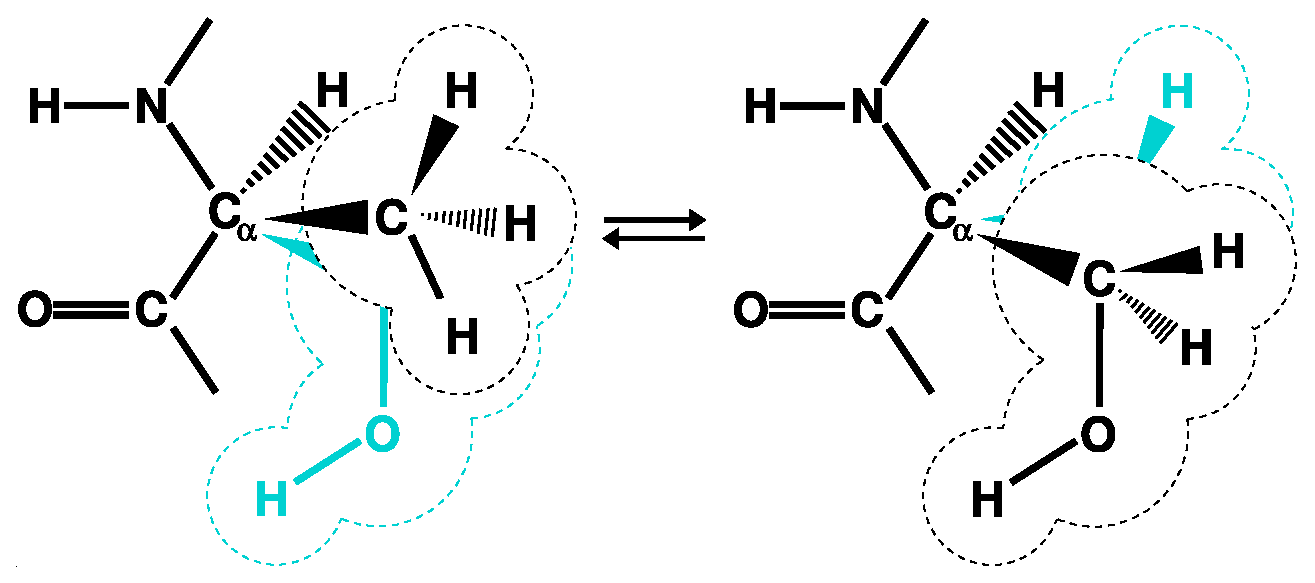
\includegraphics[width=14.5cm]{figures/dual_top}}
  \caption{Dual topology description for an alchemical simulation.
         Case example of the mutation of alanine into glycine.
         The lighter color denotes the non--interacting, alternate
         state.}
  \label{fig:dual_top}
\end{figure}


The energy and forces
are defined as a function of $\lambda$, in such a fashion that 
the interaction of the methyl group of alanine with the rest of 
the protein is effective at the beginning of the simulation,
\ie $\lambda$ = 0, while
the glycine C$_\alpha$ hydrogen does not interact with the rest
of the protein, and {\it vice versa} at the end of the
simulation, \ie $\lambda$ = 1.
For intermediate values of $\lambda$, both the alanine and the glycine
side chains participate in the non--bonded interactions with the rest 
of the protein, scaled on the basis of the current value of $\lambda$.
It should be emphasized that these side chains, however,
do not interact with each other.


It is, therefore, necessary to exclude {\it explicitly} in the setup
those atoms 
that are created from those that will be annihilated in the 
course of the \FEP\ calculation (see ``A tutorial to set up 
alchemical free energy perturbation calculations in \NAMD''
available from the \NAMD\ website).


It is also worth noting that
the free energy calculation does not alter intramolecular
potentials, \ie bond stretch, valence angle deformation, torsions
{\it etc}, during the simulation.
In calculations targetted at the estimation
of free energy differences between two states characterized by
distinct environments --- \eg a ligand bound to a protein in
the first simulation,
and solvated in water, in the second --- as is the 
case for most free energy calculations that make use of a thermodynamic 
cycle, perturbation of intramolecular terms, 
\eg chemical bonds, can be safely
avoided.~\cite{Boresch.99a}



\subsubsection{Implementation of free energy perturbation in \NAMD}


The procedure implemented in \NAMD\ is particularly
adapted for performing free 
energy calculations that split the reaction path into a number of non--physical,
intermediate $\lambda$--states, or ``windows''. Separate simulations 
can be started for each window.
Alternatively, the {\sc Tcl} scripting ability of 
\NAMD\ can be employed advantageously
to perform the complete simulation in a single run.
An example making use of such script is supplied at the end 
of this section.


The following keywords can be used to control free 
energy calculations aimed at alchemical transformations. 

\begin{itemize}

\item
\NAMDCONFWDEF{fep}{ Is alchemical \FEP\ to be performed? }
{{\tt on} or {\tt off}}
{{\tt off}}
{Turns on Hamiltonian scaling and ensemble averaging for alchemical \FEP.}

\item
\NAMDCONF{lambda}{ Coupling parameter value }
{positive decimal between 0.0 and 1.0}
{The coupling parameter value determining the progress of the
perturbation. The non--bonded interactions involving the atoms vanishing
in the course of the MD simulation are scaled by (1-{\tt lambda}), while
those of the growing atoms are scaled by {\tt lambda}.}

\item
\NAMDCONF{lambda2}{Coupling parameter comparison value}
{positive decimal between 0.0 and 1.0}
{The {\tt lambda2} value corresponds to the coupling parameter to be
used for sampling in the next window.  The free energy difference
between {\tt lambda2} and {\tt lambda} is calculated.  Through simulations
at progressive values of {\tt lambda} and {\tt lambda2} the total free
energy difference may be determined.}

\item
\NAMDCONFWDEF{fepEquilSteps}{Number of equilibration steps in the window, 
before data collection}
{positive integer less than {\tt numSteps} or {\tt run}}
{0}
{In each window {\tt fepEquilSteps} steps of equilibration can be
performed before ensemble averaging is initiated. The output also contains
the data gathered during equilibration and is meant for analysis of
convergence properties of the \FEP\ calculation.}

\item
\NAMDCONFWDEF{fepFile}{{\tt pdb} file with perturbation flags}
{filename}
{coordinates}
{{\tt pdb} file to be used for indicating the \FEP\ status for each of
the atoms pertaining to the system. 
If this parameter is not declared specifically, then the
{\tt pdb} file containing the initial coordinates specified by
{\tt coordinates} is utilized for this information.}

\item
\NAMDCONFWDEF{fepCol}{Column in the {\tt fepFile} that carries 
                      the perturbation flag}
{X, Y, Z, O or B}
{B}
{Column of the {\tt pdb} file to use for retrieving the \FEP\ status 
of each atom, \ie a flag that indicates which atom will be perturbed
in the course of the simulation.
A value of {\tt -1} in the specified column indicates the atom will
vanish during the \FEP\ calculation, whereas a value of {\tt 1} 
indicates that the atom will grow.}

\item
\NAMDCONFWDEF{fepOutFreq}{Frequency of \FEP\ energy output in time--steps}
{positive integer}
{5}
{Every {\tt fepOutFreq} number of MD steps, the output file
{\tt fepOutFile} is updated by dumping energies that are
used for ensemble averaging.
This variable could be set to {\tt 1} to include all the 
configurations for ensemble averaging. Yet, it is recommended
to update {\tt fepOutFile}  energies at longer intervals
to avoid large correlation between consecutive configurations.}

\item
\NAMDCONFWDEF{fepOutFile}{\FEP\ energy output filename}
{filename}
{outfilename}
{An output file named {\tt fepOutFile}.fep, generated by \NAMD,
contains the \FEP\ energies, dumped every {\tt fepOutFreq} steps.}

\item
\NAMDCONFWDEF{fepVdWShiftCoeff}{\FEP\ radius-shifting coefficient}
{positive decimal}
{5.}
{This is a radius-shifting coefficient of $\lambda$ that is used 
to construct the modified vdW interactions during alchemical FEP. Providing a positive value for {\tt fepVdWShiftCoeff} ensures that the vdW potential is finite everywhere for small values of $\lambda$, which significantly improves the accuracy and convergence of FEP calculations, and also prevents overlapping particles from making the simulation unstable. During FEP, the inter-atomic distances used in the Lennard-Jones potential are shifted
according to: \\
$r^2 \rightarrow r^2 + {\rm fepVdWShiftCoeff} \times (1. - \lambda)$
}

\item
\NAMDCONFWDEF{fepVdwScaleExp}{\FEP\ Lennerd-Jones parameter scaling exponent}
{decimal}
{0.}
{When constructing the modified vdW interactions during alchemical FEP, the Lennard-Jones parameters are scaled according to:\\
$A \rightarrow A \times \lambda^{2 \times {\rm fepVdwScaleExp}}$ \\
$B \rightarrow B \times \lambda^{\rm fepVdwScaleExp}$
}

%\item
%\NAMDCONFWDEF{fepElecLambdaDelay}{\FEP\ lambda ``delay" for electrostatics}
%{positive decimal}
%{0.}
%{In order to avoid the FEP ``end-point catastrophe", it is often important to make sure that a growing particle does not have an unbounded potential right when it is created (in case that it appears on top of another particle). One way to deal with this for electrostatic interactions, is to allow a bounded scaled vdW potential (using a positive fepVdWShiftCoeff) to first repel all overlapping particles at low values of $\lambda$. As $\lambda$ increases, once the particles are repelled, it is now safe to turn on FEP electrostatics. fepElecLambdaDelay is the value of $\lambda$ at which electrostatic interactins are turned on and start ramping up linearly.}


\end{itemize}


\noindent
{\it Note}: Free energy calculations that rely upon equation~({\ref{master}})
make use of an average temperature, which, in principle, should coincide with
the value of the thermostat. Rather than employing the computed average of $T$,
$\Delta A_{a \rightarrow b}$ is estimated with the target value of the
temperature defined by the user. It is, therefore, necessary to activate
some constant--temperature scheme to carry out \FEP\ calculations. 



\subsubsection{Example of an input file for running \FEP\ alchemical transformations}


The following example illustrates the use of {\sc Tcl} scripting for running
the alchemical \FEP\ feature of \NAMD: 

\begin{verbatim}
fep		on  
fepfile		ion.fep
fepCol		X
fepOutfile	ion.fepout
fepOutFreq	5
fepEquilSteps	5000

set step 0.0
set dstep 0.1

while {$step <= 0.9} {
 lambda $step
 set step [expr $step+$dstep]
 lambda2 $step
 run  10000
}
\end{verbatim}

\noindent
Here, the {\tt pdb} file read by \NAMD\ to extract the information
about perturbed atoms is {\tt biotin.fep}. The pertinent information 
is present in the {\tt X} column. The output file of the free energy
calculation is {\tt biotinr.fepout}, in which energies are written
every {\tt 5} steps.
$\delta \lambda$, the width of the windows, is set to {\tt 0.1}.
{\tt 5000} MD steps are performed in each window to
equilibrate the system. In this particular instance, 
the current value of $\lambda$
is controlled by the statement {\tt set step}. 
The \FEP\ calculation is run until $\lambda$ reaches the
value {\tt 0.9}. In every window, {\tt 10000} MD steps
are performed.


\subsubsection{Description of \FEP\ simulation output }

The {\tt fepOutFile} contains electrostatic and van der Waals energy
data calculated at $\lambda$ and $\lambda2$, written every
{\tt fepOutFreq} steps. The column {\tt dE} is the instantaneous energy
difference for the current configuration. {\tt dE\_avg} and {\tt dG}
are the accumulated energy ensemble average and the corresponding
free energy at the current time step, respectively.
The temperature is specified in the penultimate column. Upon completion
of {\tt fepEquilSteps} steps, the calculation of {\tt dE\_avg} and 
{\tt dG} is restarted. The accumulated net free energy change is output
at each $\lambda$--value and at the end of the simulation. The cumulative
average energy {\tt dE\_avg} value may be summed using, for instance, the 
trapezoidal rule, or a Gaussian quadrature, to obtain an approximate 
TI estimate for the free energy change during the run.





\subsection{Locally Enhanced Sampling}
\label{section:les}

Locally enhanced sampling (LES)~\cite{ROIT91,SIMM98,SIMM00} increases
sampling and transition rates for a portion of a molecule by the use of
multiple non-interacting copies of the enhanced atoms.  These enhanced
atoms experience an interaction (electrostatics, van der Waals, and
covalent) potential that is divided by the number of copies present.
In this way the enhanced atoms can occupy the same space, while the
multiple instances and reduces barriers increase transition rates.

\subsubsection{Structure Generation}

To use LES, the structure and coordinate input files must be modified to
contain multiple copies of the enhanced atoms.  \PSFGEN\ provides the
{\tt multiply} command for this purpose.  \NAMD\ supports a maximum of 15
copies, which should be sufficient.  

Begin by generating the complete molecular structure and guessing
coordinates as described in Sec.~\ref{section:psfgen}.  As the last
operation in your script, prior to writing the psf and pdb files, add
the {\tt multiply} command, specifying the number of copies desired and
listing segments, residues, or atoms to be multiplied.  For example,
\verb#multiply 4 BPTI:56 BPTI:57# will create four copies of the last
two residues of segment BPTI.  You must include all atoms to be
enhanced in a single {\tt multiply} command in order for the bonded
terms in the psf file to be duplicated correctly.  Calling {\tt multiply}
on connected sets of atoms multiple times will produce unpredictable
results, as may running other commands after {\tt multiply}.

The enhanced atoms are duplicated exactly in the structure---they have
the same segment, residue, and atom names.  They are distinguished only
by the value of the B (beta) column in the pdb file, which is 0 for
normal atoms and varies from 1 to the number of copies created for
enhanced atoms.  The enhanced atoms may be easily observed in VMD with
the atom selection \verb#beta != 0#.

\subsubsection{Simulation}

In practice, LES is a simple method used to increase sampling;
no special output is generated.
The following parameters are used to enable LES:

\begin{itemize}

\item
\NAMDCONFWDEF{les}{is locally enhanced sampling active?}{{\tt on} or {\tt
off}}{{\tt off}}
{Specifies whether or not LES is active.}

\item
\NAMDCONF{lesFactor}{number of LES images to use}
{positive integer equal to the number of images present}
{This should be equal to the factor used in {\tt multiply}
 when creating the structure.  The interaction potentials for images is
 divided by {\tt lesFactor}.  
}

\item
\NAMDCONFWDEF{lesFile}{PDB file containing LES flags}{UNIX filename} {{\tt coordinates}}
{PDB file to specify the LES image number of each atom.
If this parameter is not specified, then 
the PDB file containing initial coordinates specified by 
{\tt coordinates} is used.}

\item
\NAMDCONFWDEF{lesCol}{column of PDB file containing LES flags}{{\tt X}, {\tt Y}, {\tt Z}, {\tt O}, or {\tt B}}{{\tt B}}
{Column of the PDB file to specify the LES image number of each atom.
This parameter may specify any of the floating point fields of the PDB file, 
either X, Y, Z, occupancy, or beta-coupling (temperature-coupling).  
A value of 0 in this column indicates that the atom is not enhanced.
Any other value should be a positive integer less than {\tt lesFactor}.}

\end{itemize}

The parameter {\tt lesFactor} may be varied between simulations to
interpolate between full enhancement and normal simulation (although
multiple bonded images are present at all times).  If {\tt lesFactor}
is decreased, the images with flags greater than {\tt lesFactor} will
be decoupled from nonbonded terms, sample based only on bonded terms,
and should therefore be excluded from analysis.  When increasing
{\tt lesFactor} the coordinates of these abandoned images should be
reset to that of another image to avoid any bad initial contacts and
the resulting instability in the simulation.

\subsection{Pair Interaction Calculations}
\NAMD supportes the calculation of nonbonded interaction energies between 
two groups of atoms.  When enabled, pair interaction information will be
calculated and printed in the standard output file on its own line at the
same frequency as energy output.  The format of the line is
{\tt PAIR INTERACTION: STEP: {\it step} VDW: {\it vdw} FORCE: {\it fx fy fz}}.
The displayed force is the force on atoms in group 1.

For trajectory analysis the 
recommended way to use this set of options is to use the NAMD Tcl scripting 
interface as described in Sec.~\ref{section:tclscripting} to run for
0 steps, so that NAMD prints the energy without performing any dynamics.

\begin{itemize}

\item
\NAMDCONFWDEF{pairInteraction}{is pair interaction calculation active?}
{{\tt on} or {\tt off}}{{\tt off}}
{Specifies whether pair interaction calculation is active.}

\item
\NAMDCONFWDEF{pairInteractionFile}{PDB file containing pair interaction flags}
{UNIX filename}{{\tt coordinates}}
{PDB file to specify atoms to use for pair interaction calculations.  If 
this parameter is not specified, then the PDB file containing initial 
coordinates specified by {\tt coordinates} is used.}

\item
\NAMDCONFWDEF{pairInteractionCol}{column of PDB file containing pair 
interaction flags}{{\tt X}, {\tt Y}, {\tt Z}, {\tt O}, or {\tt B}}{{\tt B}}
{
Column of the PDB file to specify which atoms to use for pair interaction
calculations.  This parameter may specify any of the floating point
fields of the PDB file, either X, Y, Z, occupancy, or beta-coupling
(temperature-coupling).  A value of zero in this column indicates the atom
is not involved in pair interaction calculations; a value of -1 indicates it
belongs to group 1; a value of 2 indicates it belongs to group 2.
}

\item
\NAMDCONFWDEF{pairInteractionOnly}{should only pair interactions be 
calculated?}{{\tt yes} or {\tt no}}{{\tt no}}
{ Specifies whether to compute only pair interaction calculations and nothing
else.  Choose {\tt yes} when analyzing completed trajectories; choose {\tt no}
to output pair interaction energies while the simulation is running.}

